\documentclass[a4paper,12pt]{extarticle}
\usepackage[utf8x]{inputenc}
\usepackage[T1,T2A]{fontenc}
\usepackage[russian]{babel}
\usepackage[hidelinks]{hyperref}
\usepackage{indentfirst}
\usepackage{listings}
\usepackage{color}
\usepackage{here}
\usepackage{array}
\usepackage{multirow}
\usepackage{graphicx}
\usepackage{subcaption} 
\usepackage{mathtools}

\usepackage{caption}
\renewcommand{\lstlistingname}{Программа} % заголовок листингов кода

\bibliographystyle{ugost2008ls}

\usepackage{listings}
\lstset{ %
extendedchars=\true,
keepspaces=true,
language=C,						% choose the language of the code
basicstyle=\footnotesize,		% the size of the fonts that are used for the code
numbers=left,					% where to put the line-numbers
numberstyle=\footnotesize,		% the size of the fonts that are used for the line-numbers
stepnumber=1,					% the step between two line-numbers. If it is 1 each line will be numbered
numbersep=5pt,					% how far the line-numbers are from the code
backgroundcolor=\color{white},	% choose the background color. You must add \usepackage{color}
showspaces=false				% show spaces adding particular underscores
showstringspaces=false,			% underline spaces within strings
showtabs=false,					% show tabs within strings adding particular underscores
frame=single,           		% adds a frame around the code
tabsize=2,						% sets default tabsize to 2 spaces
captionpos=t,					% sets the caption-position to top
breaklines=true,				% sets automatic line breaking
breakatwhitespace=false,		% sets if automatic breaks should only happen at whitespace
escapeinside={\%*}{*)},			% if you want to add a comment within your code
postbreak=\raisebox{0ex}[0ex][0ex]{\ensuremath{\color{red}\hookrightarrow\space}},
texcl=true,
inputpath=listings,                     % директория с листингами
}

\usepackage[left=2cm,right=2cm,
top=2cm,bottom=2cm,bindingoffset=0cm]{geometry}

%% Нумерация картинок по секциям
\usepackage{chngcntr}
\counterwithin{figure}{section}
\counterwithin{table}{section}

%%Точки нумерации заголовков
\usepackage{titlesec}
\titlelabel{\thetitle.\quad}
\usepackage[dotinlabels]{titletoc}

%% Оформления подписи рисунка
\addto\captionsrussian{\renewcommand{\figurename}{Рисунок}}
\captionsetup[figure]{labelsep = period}

%% Подпись таблицы
%\DeclareCaptionFormat{hfillstart}{\hfill#1#2#3\par}
%\captionsetup[table]{format=hfillstart,labelsep=newline,justification=centering,skip=-10pt,textfont=bf}

%% Путь к каталогу с рисунками
\graphicspath{{fig/}}

%% Внесение titlepage в учёт счётчика страниц
\makeatletter
\renewenvironment{titlepage} {
 \thispagestyle{empty}
}
\makeatother

\DeclarePairedDelimiter\abs{\lvert}{\rvert}%
\DeclarePairedDelimiter\norm{\lVert}{\rVert}%

\usepackage{amsmath}

\begin{document}	% начало документа

% Титульная страница
\begin{titlepage}	% начало титульной страницы

	\begin{center}		% выравнивание по центру

		\large Санкт-Петербургский политехнический университет Петра Великого\\
		\large Институт прикладной математики и механики \\
		\large Кафедра <<Прикладная математика>>\\[6cm]
		% название института, затем отступ 6см
		
		\huge Математическая статистика\\[0.5cm] % название работы, затем отступ 0,5см
		%\huge Методы оптимизации\\[0.5cm] % название работы, затем отступ 0,5см
		\large \textbf{Отчет по лабораторной работе №4}\\[5.1cm]
		%\large \textbf{Отчет по лабораторной работе \\``Решение задач одномерной минимизации ``}\\[5.1cm]
		%\\[5cm]

	\end{center}


	\begin{flushright} % выравнивание по правому краю
		\begin{minipage}{0.25\textwidth} % врезка в половину ширины текста
			\begin{flushleft} % выровнять её содержимое по левому краю

				\large\textbf{Работу выполнил:}\\
				\large Колесник В.Н.\\
				\large {Группа:} 3630102/70201\\
				
				\large \textbf{Преподаватель:}\\
				\large к.ф.-м.н., доцент\\
				\large Баженов Александр Николаевич
				%\large Родионова Елена Александровна

			\end{flushleft}
		\end{minipage}
	\end{flushright}
	
	\vfill % заполнить всё доступное ниже пространство

	\begin{center}
	\large Санкт-Петербург\\
	\large \the\year % вывести дату
	\end{center} % закончить выравнивание по центру

\end{titlepage} % конец титульной страницы

\vfill % заполнить всё доступное ниже пространство


% Содержание
\renewcommand\contentsname{\centerline{Содержание}}
\tableofcontents
\newpage

\listoffigures
\newpage

\listoftables
\newpage

\section{Постановка задачи}
Для 5 распределений:
\begin{itemize}
\item Нормальное распределение  \(N(x, 0, 1)\)
\item Распределение Коши  \(C(x, 0, 1)\)
\item Распределение Лапласа  \(L(x, 0, \frac{1}{\sqrt{2}})\)
\item Распределение Пуассона  \(P(k, 10)\)
\item Равномерное распределение  \(U(x, -\sqrt{3}, \sqrt{3})\)
\end{itemize}
Сгенерировать выборки размером 20, 60 и 100 элементов. \\
Построить на них эмпирические функции распределения и ядерные
оценки плотности распределения на отрезке [−4; 4] для непрерывных
распределений и на отрезке [6; 14] для распределения Пуассона.

\section{Теория}
\subsection{Распределения}
\begin{itemize}
\item Нормальное распределение
\begin{equation}
N(x, 0, 1)=\frac{1}{\sqrt{2\pi}}e^{\frac{-x^2}{2}}
\end{equation}
\item Распределение Коши
\begin{equation}
C(x, 0, 1)=\frac{1}{\pi}\frac{1}{x^2+1}
\end{equation}
\item Распределение Лапласа
\begin{equation}
L(x, 0, \frac{1}{\sqrt{2}})=\frac{1}{\sqrt{2}}e^{-\sqrt{2}| x |}
\end{equation}
\item Распределение Пуассона
\begin{equation}
P(k, 10)=\frac{10^k}{k!}e^{-10}
\end{equation}
\item Равномерное распределение
\begin{equation}
U(x, -\sqrt{3}, \sqrt{3})=
\left\{
  \begin{array}{lr}
    \frac{1}{2\sqrt{3}} & | x | \leq \sqrt{3}\\
    0 & | x | > \sqrt{3}
  \end{array}
\right.
\end{equation}
\end{itemize}



\subsection{Эмпирическая функция распределения}
\subsubsection{Статистический ряд}
Статистическим рядом называется последовательность различных элементов выборки \(z_1, z_2, ..., z_k\), расположенных в возрастающем порядке с указанием частот \(n_1, n_2, ..., n_k\), с которыми эти элементы содержатся в выборке.\\
Статистический ряд обычно записывается в виде таблицы

\begin{table}[!htb]
\centering
\label{tab:tab1}
\begin{tabular}{|c|c|c|c|c|}
\hline
\(z\) &\(z_1\) & \(z_2\)&...& \(z_k\)\\
\hline
\(n\) &\(n_1\) & \(n_2\)&...& \(n_k\)\\
\hline
\end{tabular}
\centering
\caption{Статистический ряд}
\end{table}


\subsubsection{Определение}
Эмпирической (выборочной) функцией распределения (э. ф. р.) называется относительная частота события \(X<x\), полученная по данной выборке:
\begin{equation}\label{def}
F^*_n (x) = P^* (X<x)
\end{equation}


\subsubsection{Описание}
Для получения относительной частоты \(P^\ast(X<x)\) просуммируем в статистическом ряде, построенном по данной выборке, все частоты \(n_i\), для которых элементы \(z_i\) статистического ряда меньше \(x\). Тогда \(P^\ast(X<x)=\frac{1}{n}\sum_{z_i <x} n_i.\) Получаем
\begin{equation}\label{descr}
F^\ast(x)=\frac{1}{n}\sum_{z_i <x} n_i.
\end{equation}
\(F^\ast(x)\) - функция распределения дискретной случайной величины \(X^\ast\), заданной таблицей распределения
\begin{table}[!htb]
\centering
\label{tab:tab2}
\begin{tabular}{|c|c|c|c|c|}
\hline
\(X^\ast\) &\(z_1\) & \(z_2\)&...& \(z_k\)\\
\hline
\(P\) &\(\frac{n_1}{n}\) & \(\frac{n_2}{n}\)&...& \(\frac{n_k}{n}\)\\
\hline
\end{tabular}
\centering
\caption{Таблица распределений}
\end{table}
Эмпирическая функция распределения является оценкой, т. е. приближённым значением, генеральной функции распределения
\begin{equation}\label{descr2}
F^\ast_n(x)\approx F_X(x).
\end{equation}



\subsection{Оценки плотности вероятности}
\subsubsection{Определение}
Оценкой плотности вероятности \(f(x)\) называется функция \(\widehat{f}(x)\), построенная на основе выборки, приближённо равная \(f(x)\)
\begin{equation}\label{def2}
\widehat{f}(x)\approx f(x).
\end{equation}

\subsubsection{Ядерные оценки}
Представим оценку в виде суммы с числом слагаемых, равным объёму выборки:
\begin{equation}\label{ker2}
\widehat{f}(x)=\frac{1}{n h_n} \sum_{i=1}{n} K(\frac{x - x_i}{h_n})
\end{equation}
Здесь функция \(K(u)\), называемая ядерной (ядром), непрерывна и является плотностью вероятности,  \(x_1, x_2, ..., x_n\) — элементы выборки, \(\{h_n\}\) — любая последовательность положительных чисел, обладающая свойствами
\begin{equation}\label{ker3}
h_{n} \xrightarrow[n \to \infty]{} 0;  \frac{h_{n}}{n^{-1}} \xrightarrow[n \to \infty]{} \infty.
\end{equation}
Такие оценки называются непрерывными ядерными.\\
Замечание. Свойство, означающее сближение оценки с оцениваемой величиной при \(n\to\infty\) в каком-либо смысле, называется состоятельностью оценки.\\
Если плотность \(f(x)\) кусочно-непрерывная, то ядерная оценка плотности является состоятельной при соблюдении условий, накладываемых на параметр сглаживания \(h_n\), а также на ядро \(K(u)\).\\
Гауссово (нормальное) ядро
\begin{equation}\label{ker4}
K(u)=\frac{1}{\sqrt{2\pi}}e^{-\frac{u^2}{2}}.
\end{equation}
Правило Сильвермана
\begin{equation}\label{ker5}
h_n=1.06\widehat{\sigma}n^{-\frac{1}{5}},
\end{equation}
где \(\widehat{\sigma}\) - выборочное стандартное отклонение.


\section{Реализация}
Лабораторная работа выполнена на языке программирования R в среде RStudio. Использовалась библиотека LaplaceDemon. Исходный код лабораторной привёден в приложении.



\section{Результаты}
\subsection{Эмпирические функции распределения}

\subsubsection{Нормальное распределение}
\begin{figure}[!htb]
\minipage{0.32\textwidth}
  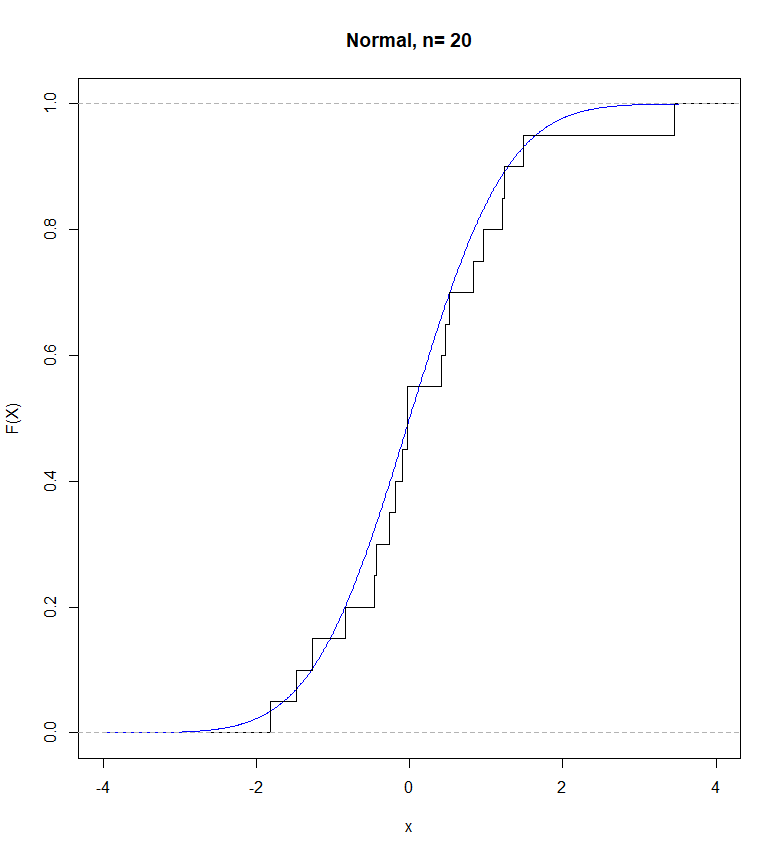
\includegraphics[width=\linewidth]{a748f443-0068-4ac7-b339-3c74bd1b2c49.png}
  \caption{Norm, n=20}
\endminipage\hfill
\minipage{0.32\textwidth}
  \includegraphics[width=\linewidth]{norm2.png}
  \caption{Norm, n=60}
\endminipage\hfill
\minipage{0.32\textwidth}
  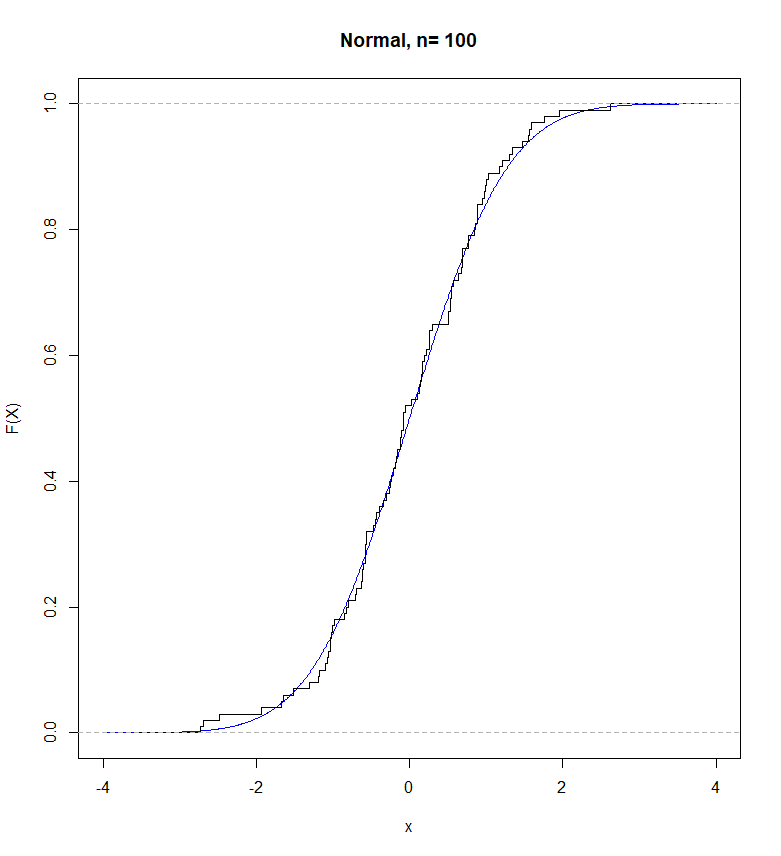
\includegraphics[width=\linewidth]{08588236-aa2a-422b-bbbb-ea571ef25b35.png}
  \caption{Norm, n=100}
\endminipage
 \label{fig:norm}
\end{figure}
\newpage
\subsubsection{Распределение Пуассона}
\begin{figure}[!htb]
\minipage{0.32\textwidth}
  \includegraphics[width=\linewidth]{pois1.png}
  \caption{Pois, n=20}
\endminipage\hfill
\minipage{0.32\textwidth}
  \includegraphics[width=\linewidth]{pois2.png}
  \caption{Pois, n=60}
\endminipage\hfill
\minipage{0.32\textwidth}
  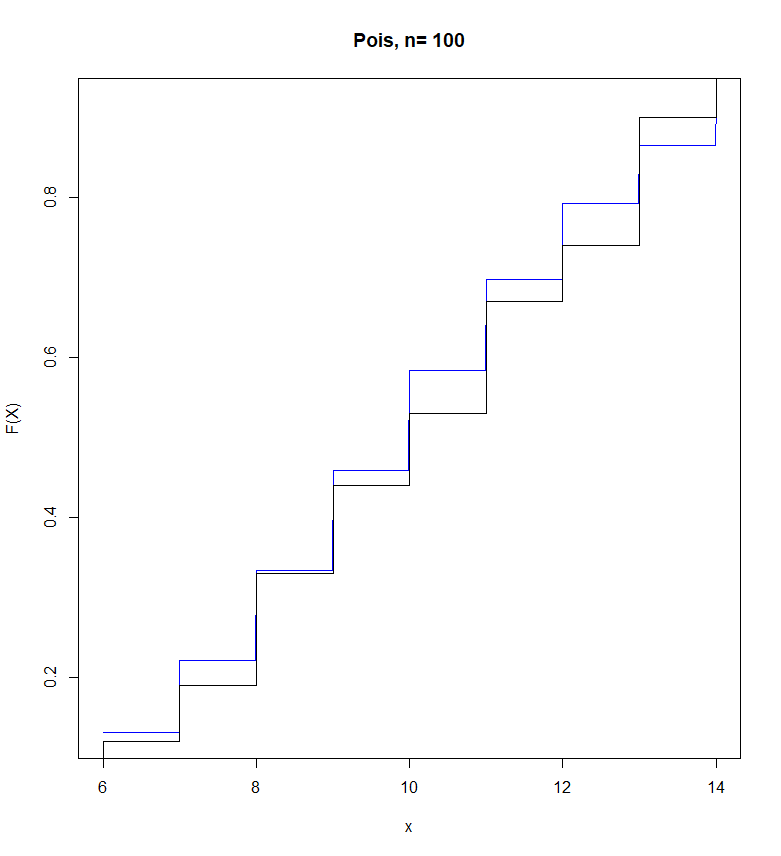
\includegraphics[width=\linewidth]{93538209-5a72-4ae8-ac85-ffa477bbb414.png}
  \caption{Pois, n=100}
\endminipage
 \label{fig:pois}
\end{figure}
\newpage
\subsubsection{Распределение Лапласа}
\begin{figure}[!htb]
\minipage{0.32\textwidth}
  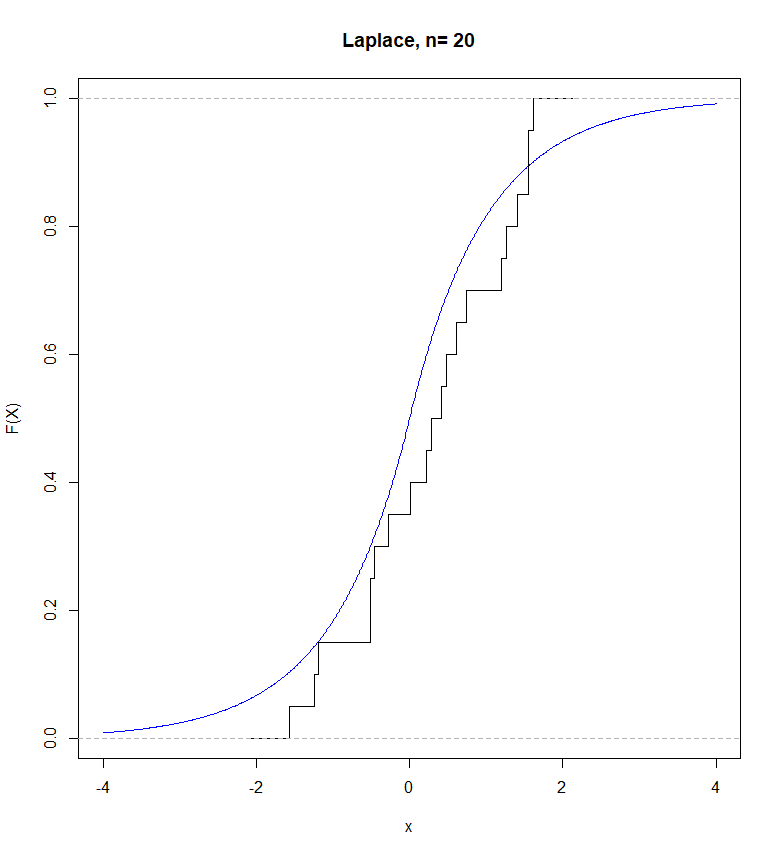
\includegraphics[width=\linewidth]{c1801c3c-fadb-45fc-8cef-562ec86574d5.png}
  \caption{Lapl, n=20}
\endminipage\hfill
\minipage{0.32\textwidth}
  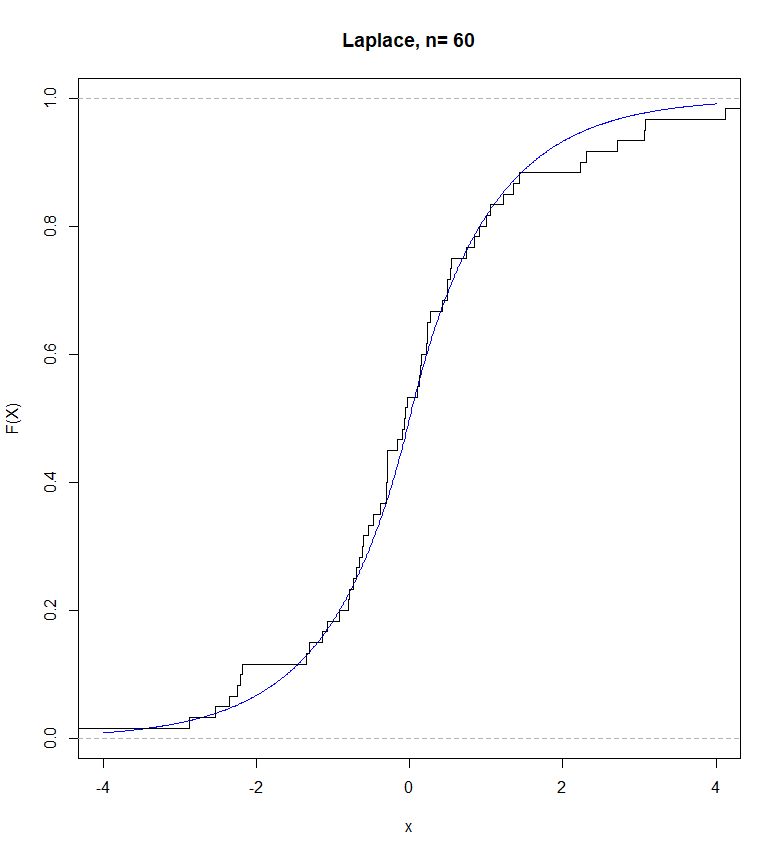
\includegraphics[width=\linewidth]{3d0f1302-6bc1-4f00-bdc5-f54be1369fc0.png}
  \caption{Lapl, n=60}
\endminipage\hfill
\minipage{0.32\textwidth}
  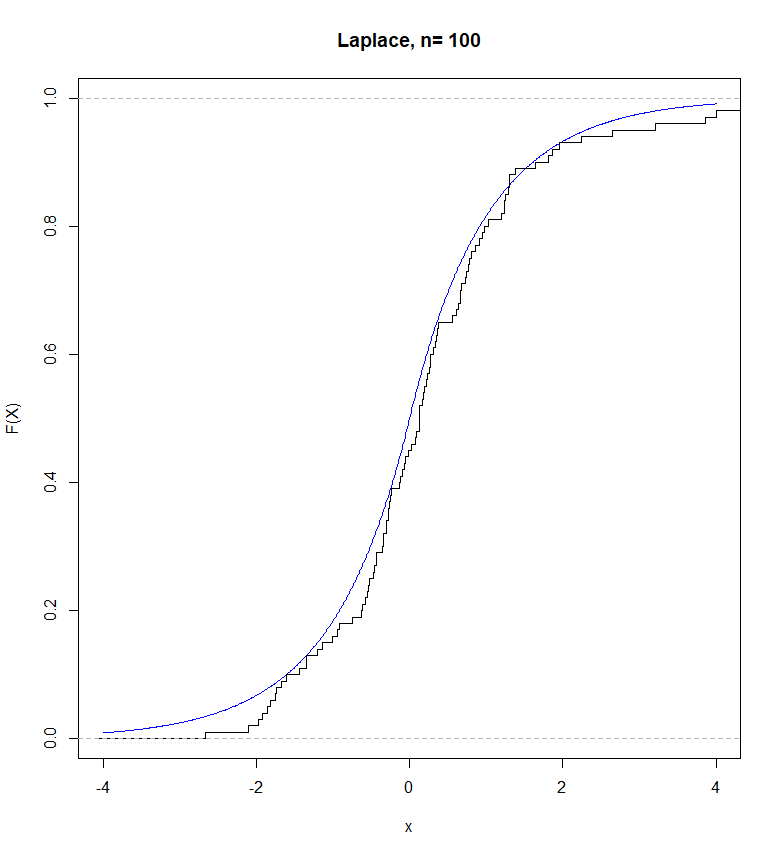
\includegraphics[width=\linewidth]{01040f4d-f009-447c-a091-8f6f8e995ed6.png}
  \caption{Lapl, n=100}
\endminipage
 \label{fig:lapl}
\end{figure}
\newpage
\subsubsection{Распределение Коши}
\begin{figure}[!htb]
\minipage{0.32\textwidth}
  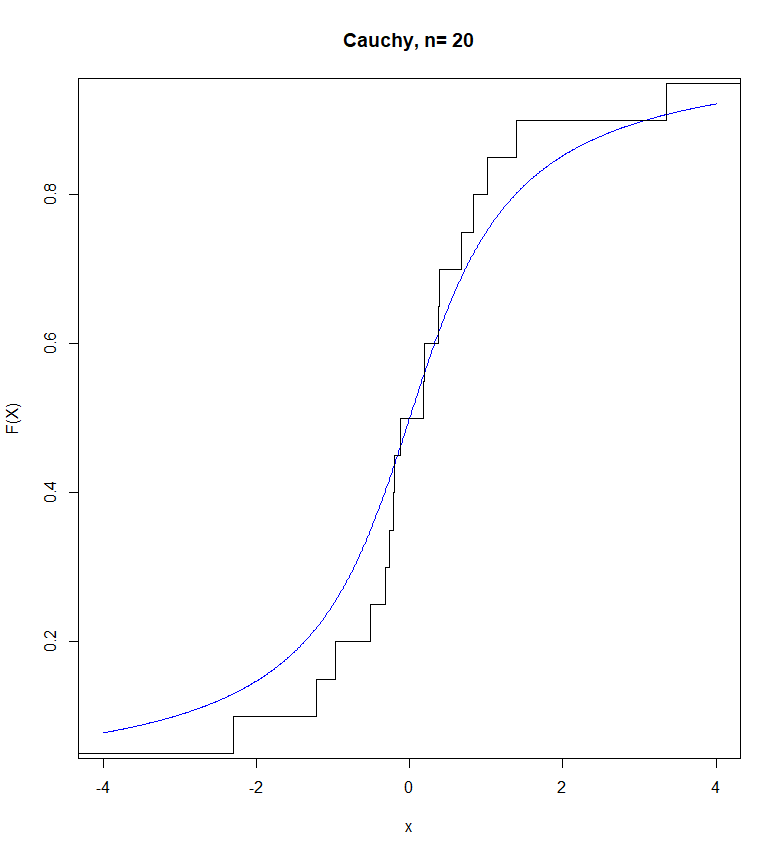
\includegraphics[width=\linewidth]{350fb4d3-91c6-49ab-afe8-8e1360521ca7.png}
  \caption{Cauchy, n=20}
\endminipage\hfill
\minipage{0.32\textwidth}
  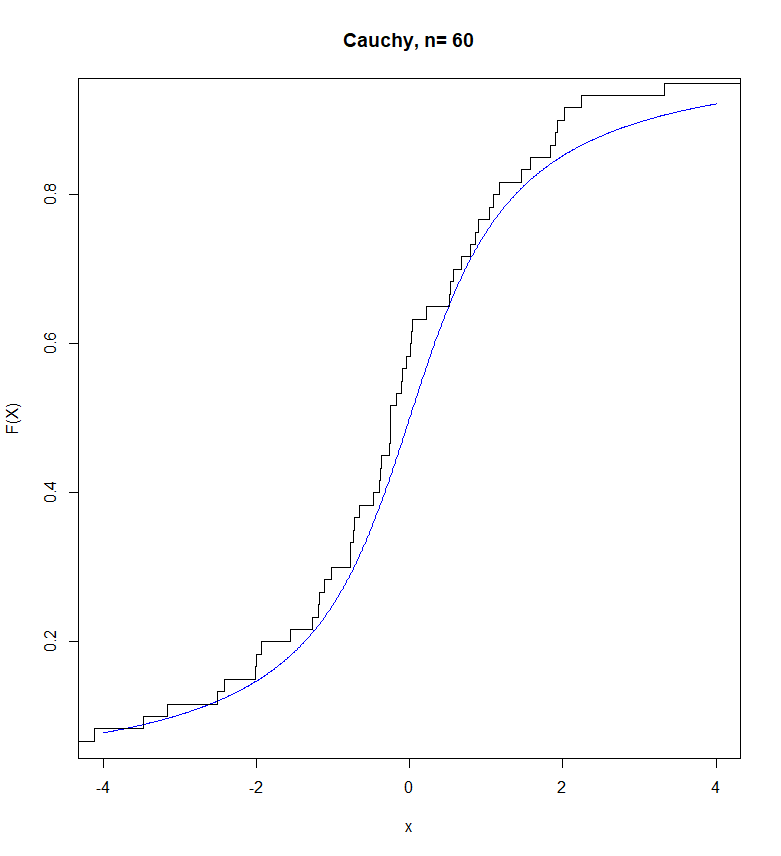
\includegraphics[width=\linewidth]{ce3daece-bafd-483c-ac62-394e2aefd931.png}
  \caption{Cauchy, n=60}
\endminipage\hfill
\minipage{0.32\textwidth}
  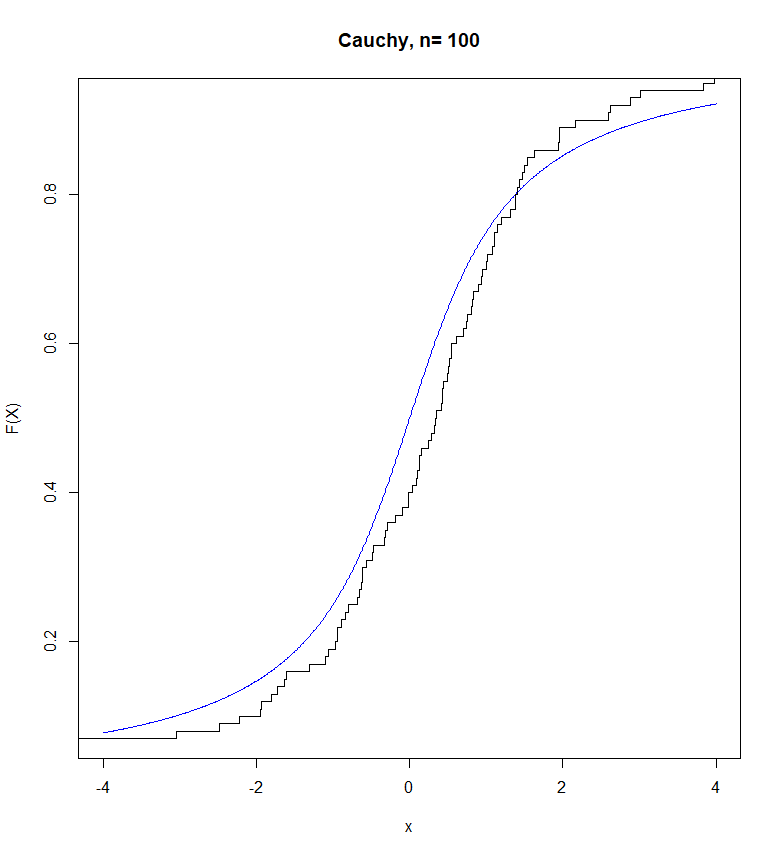
\includegraphics[width=\linewidth]{2e3bfb6c-c366-471d-aea4-5e6a5508916a.png}
  \caption{Cauchy, n=100}
\endminipage
 \label{fig:cauchy}
\end{figure}
\newpage
\subsubsection{Равномерное распределение}
\begin{figure}[!htb]
\minipage{0.32\textwidth}
  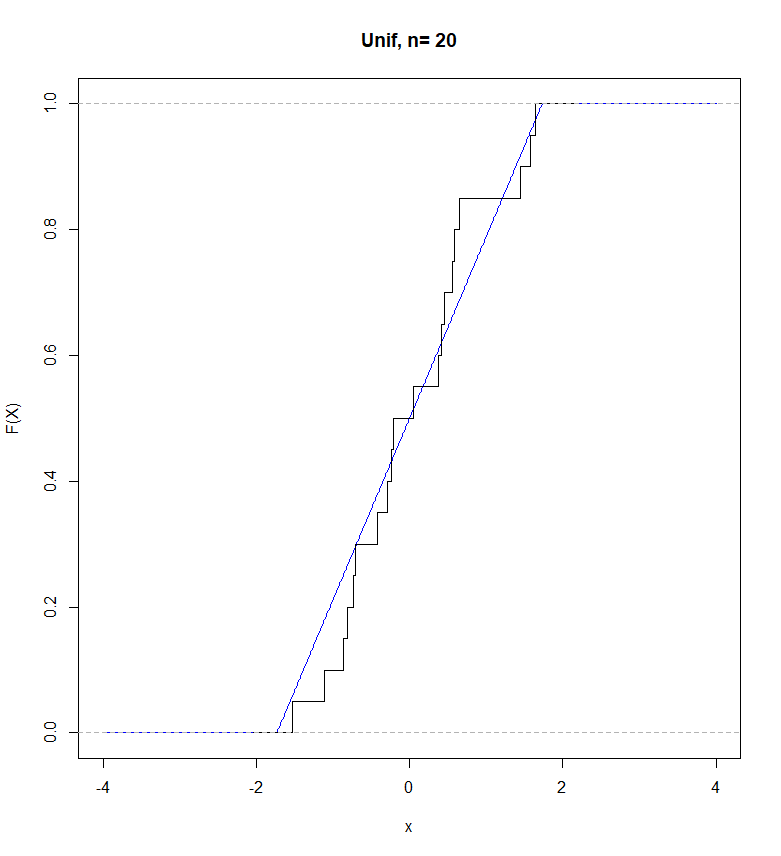
\includegraphics[width=\linewidth]{c3121468-0eaa-4fd4-9581-ebc0088c13d4.png}
  \caption{Unif, n=20}
\endminipage\hfill
\minipage{0.32\textwidth}
  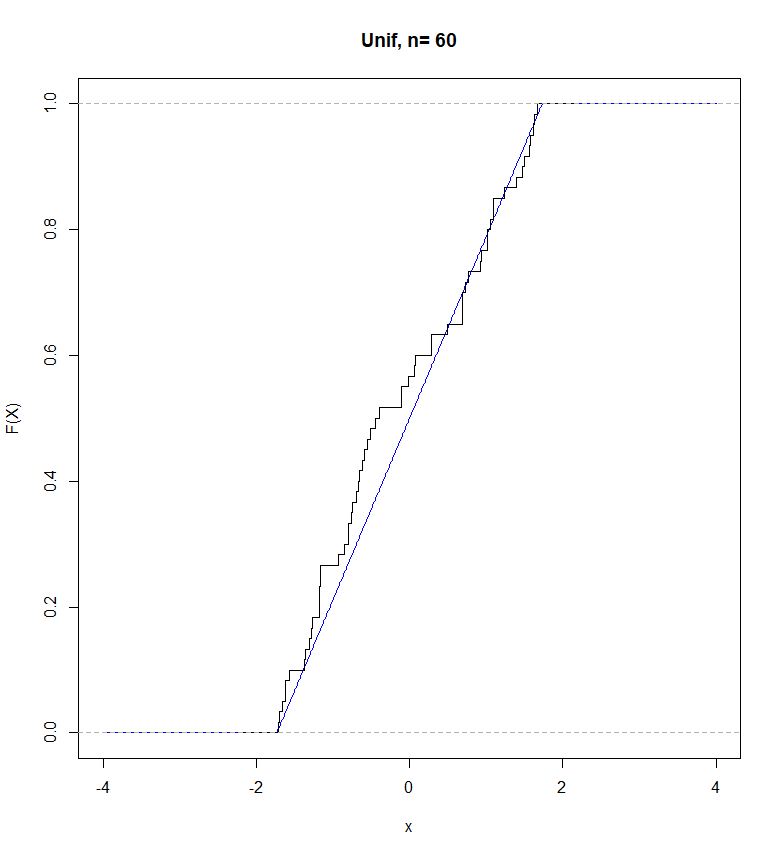
\includegraphics[width=\linewidth]{6a68a1d3-cf23-406f-8cae-1009d65169fc.png}
  \caption{Unif, n=60}
\endminipage\hfill
\minipage{0.32\textwidth}
  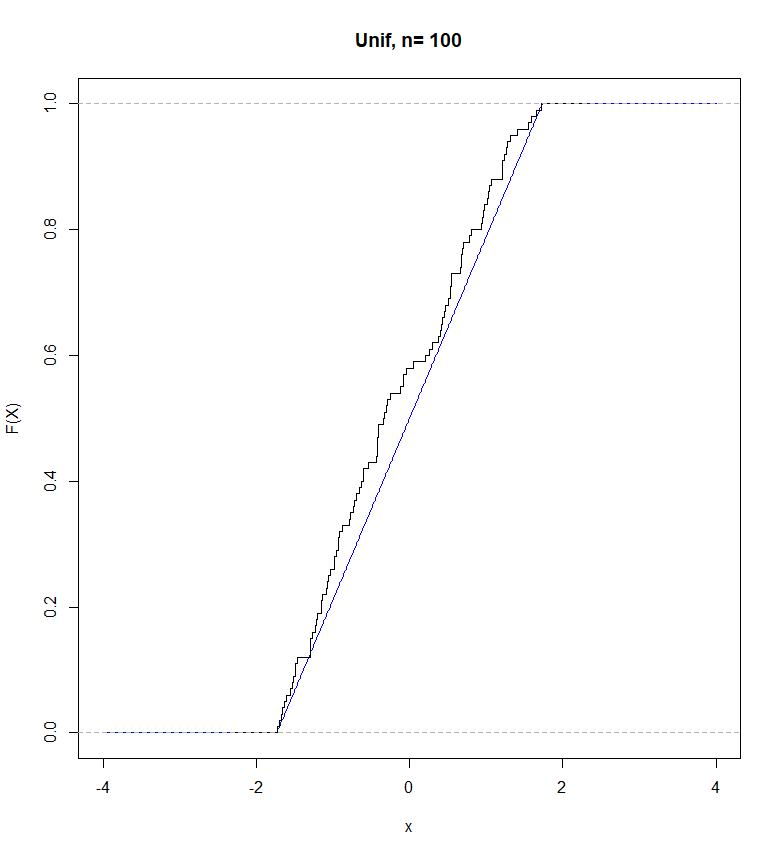
\includegraphics[width=\linewidth]{47835605-257d-4ee1-88fc-bb164b304ad7.png}
  \caption{Unif, n=100}
\endminipage
 \label{fig:unif}
\end{figure}
\newpage
\subsection{Ядерные оценки плотности распределения}%%%%%%%%%%%%%%%%%%%%%%
\subsubsection{Нормальное распределение, n = 20}
\begin{figure}[!htb]
\minipage{0.32\textwidth}
  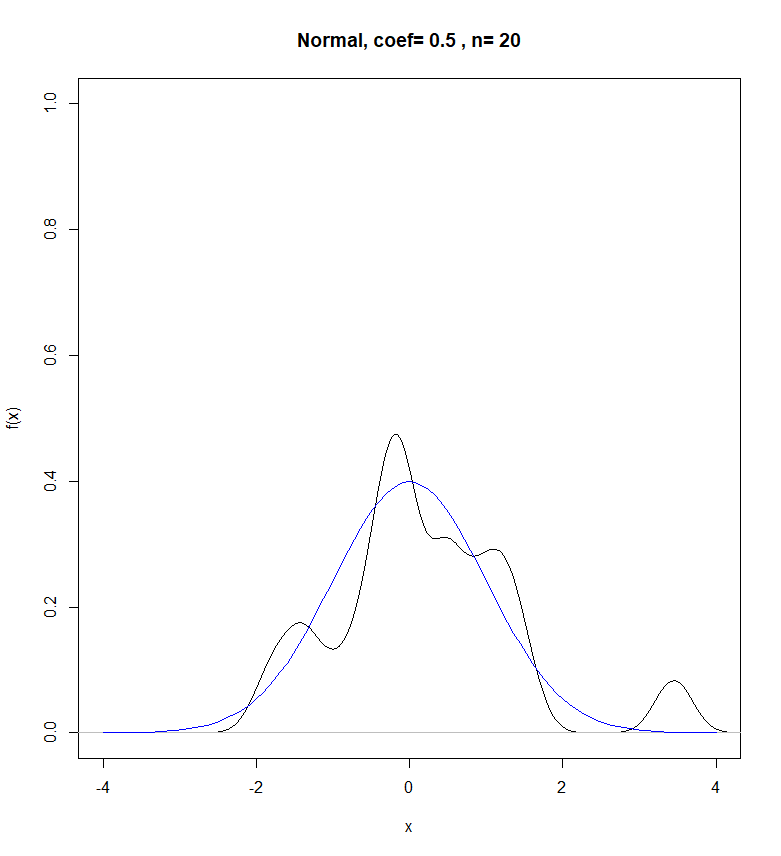
\includegraphics[width=\linewidth]{233f453d-092c-4ffb-b36c-cb4f8cd0aba7.png}
  \caption{\(Norm, h=h_n/2\)}
\endminipage\hfill
\minipage{0.32\textwidth}
  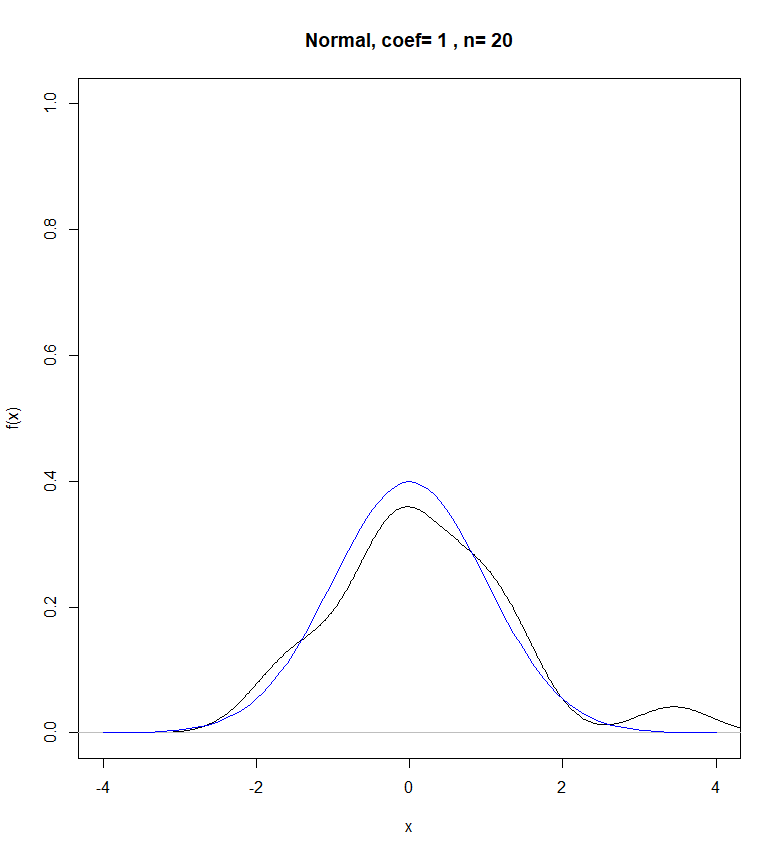
\includegraphics[width=\linewidth]{325bf7ce-7b08-4fdb-b9be-0e53b9b8e250.png}
  \caption{\(Norm, h=h_n\)}
\endminipage\hfill
\minipage{0.32\textwidth}
  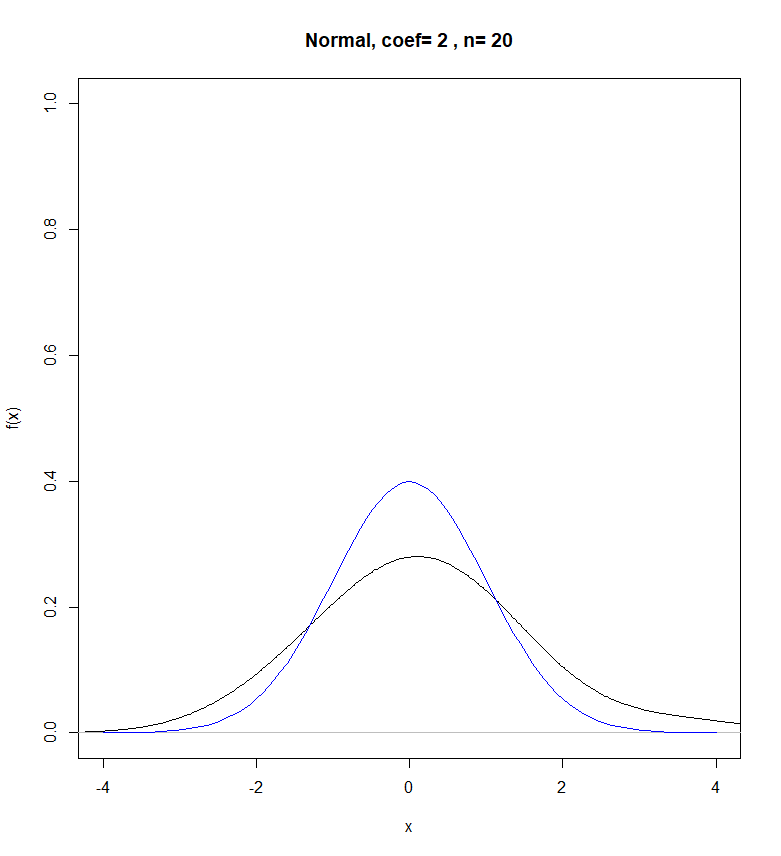
\includegraphics[width=\linewidth]{ef302f71-d0e1-48f7-b407-43c3738072f4.png}
  \caption{\(Norm, h=2h_n\)}
\endminipage
\label{fig:norm20}
\end{figure}
\subsubsection{Нормальное распределение, n = 60}
\begin{figure}[!htb]
\minipage{0.32\textwidth}
  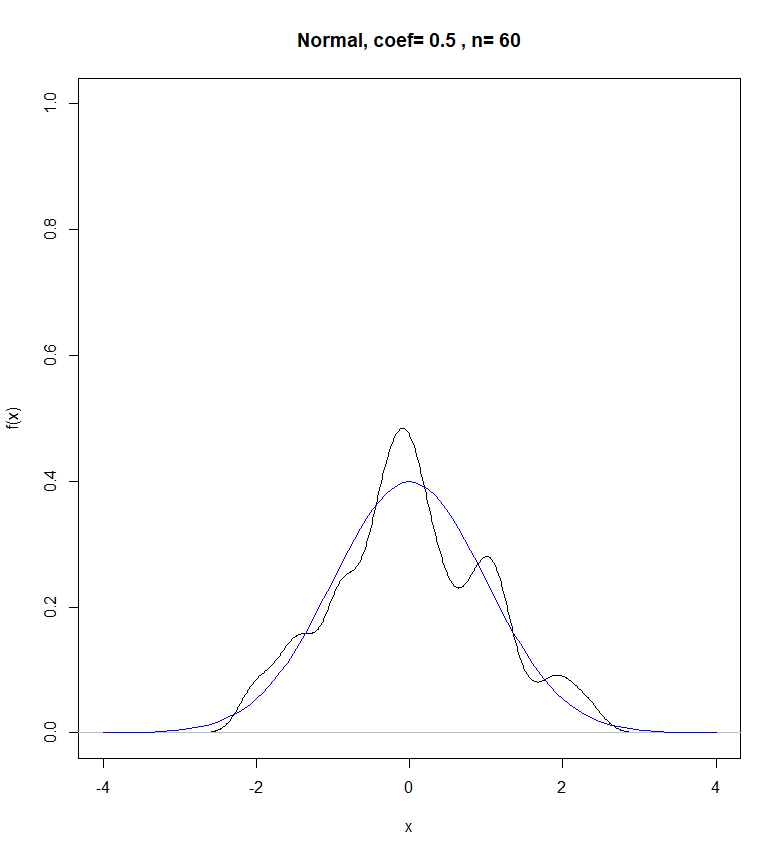
\includegraphics[width=\linewidth]{c51af086-9406-4c3f-961b-d9828117c805.png}
  \caption{\(Norm, h=h_n/2\)}
\endminipage\hfill
\minipage{0.32\textwidth}
  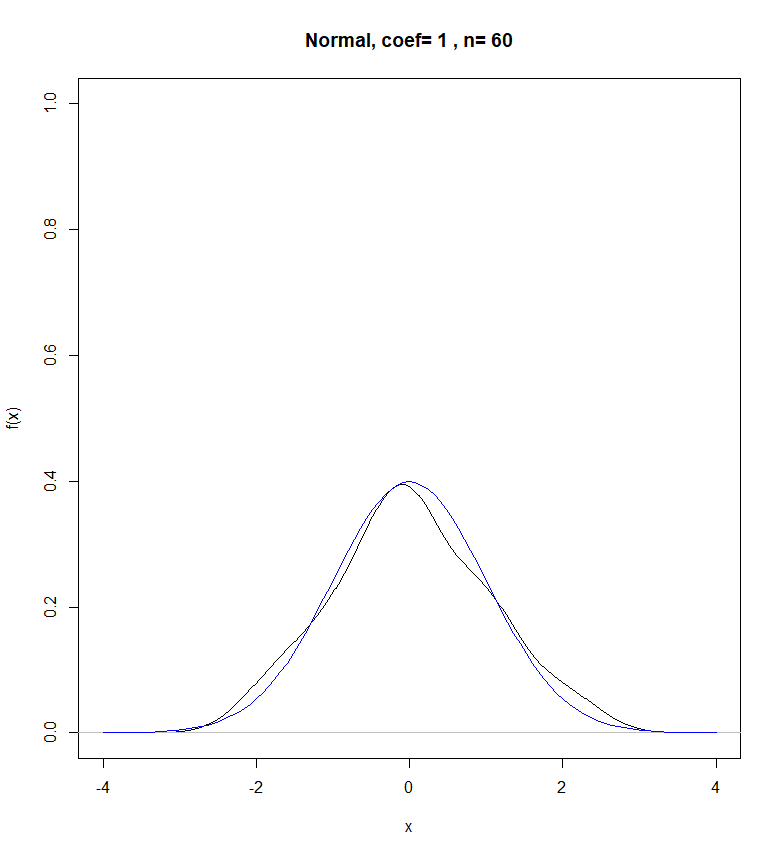
\includegraphics[width=\linewidth]{2adf5512-af32-41e6-bdc4-1cde5e01220c.png}
  \caption{\(Norm, h=h_n\)}
\endminipage\hfill
\minipage{0.32\textwidth}
  \includegraphics[width=\linewidth]{f2f70ab2-5c38-4f18-bfac-96a8f6f0b152.png}
  \caption{\(Norm, h=2h_n\)}
\endminipage
 \label{fig:norm60}
\end{figure}
\subsubsection{Нормальное распределение, n = 100}
\begin{figure}[!htb]
\minipage{0.32\textwidth}
  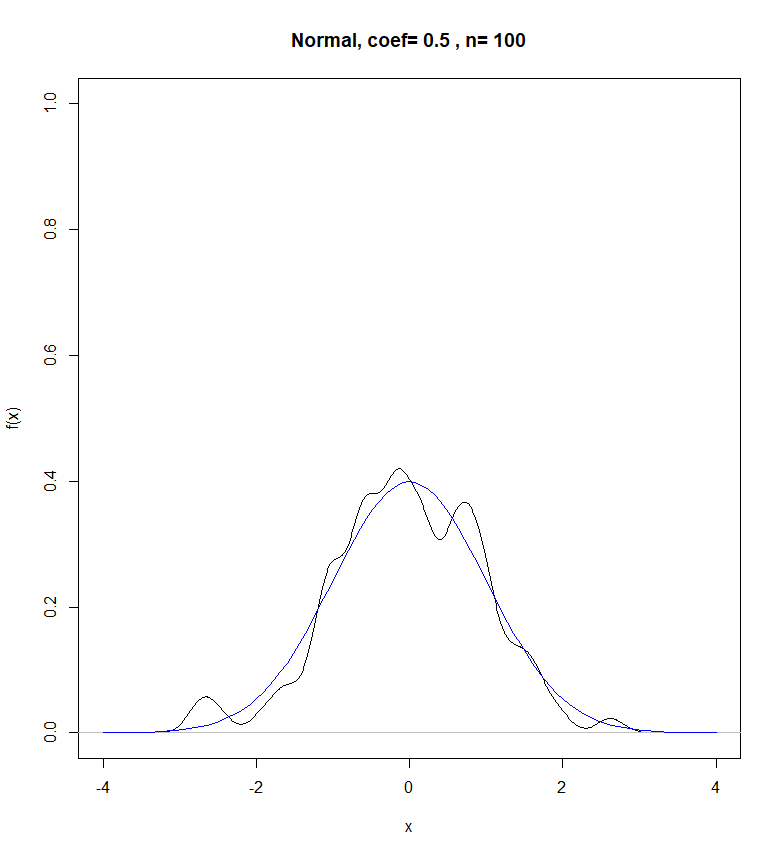
\includegraphics[width=\linewidth]{761a44bc-f20b-4d89-9fa1-462fac8b2244.png}
  \caption{\(Norm, h=h_n/2\)}
\endminipage\hfill
\minipage{0.32\textwidth}
  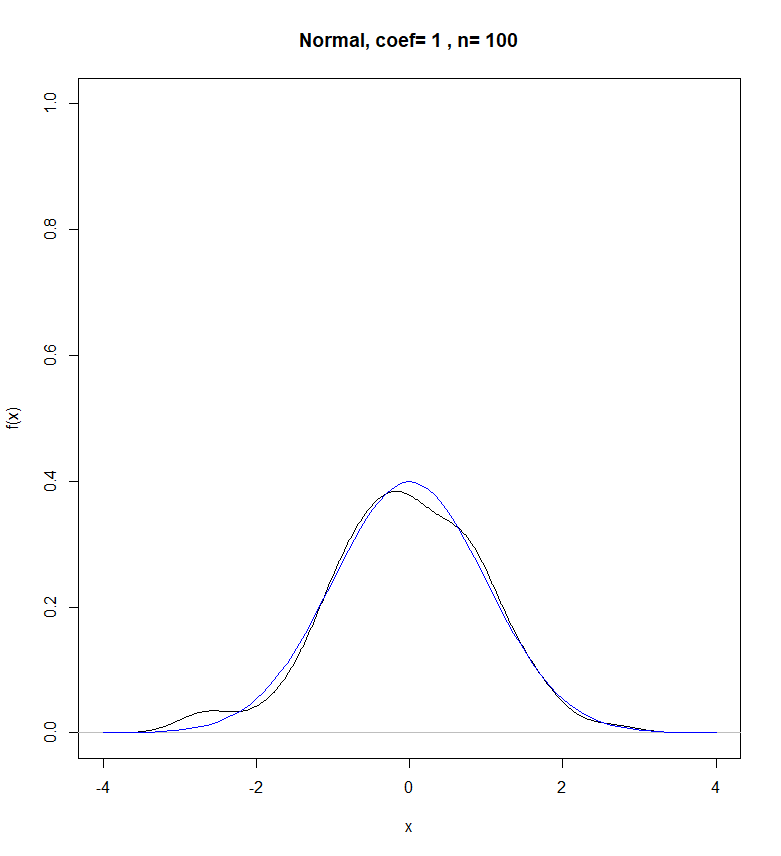
\includegraphics[width=\linewidth]{8b07ed7d-d755-4b61-810e-40782a3b2315.png}
  \caption{\(Norm, h=h_n\)}
\endminipage\hfill
\minipage{0.32\textwidth}
  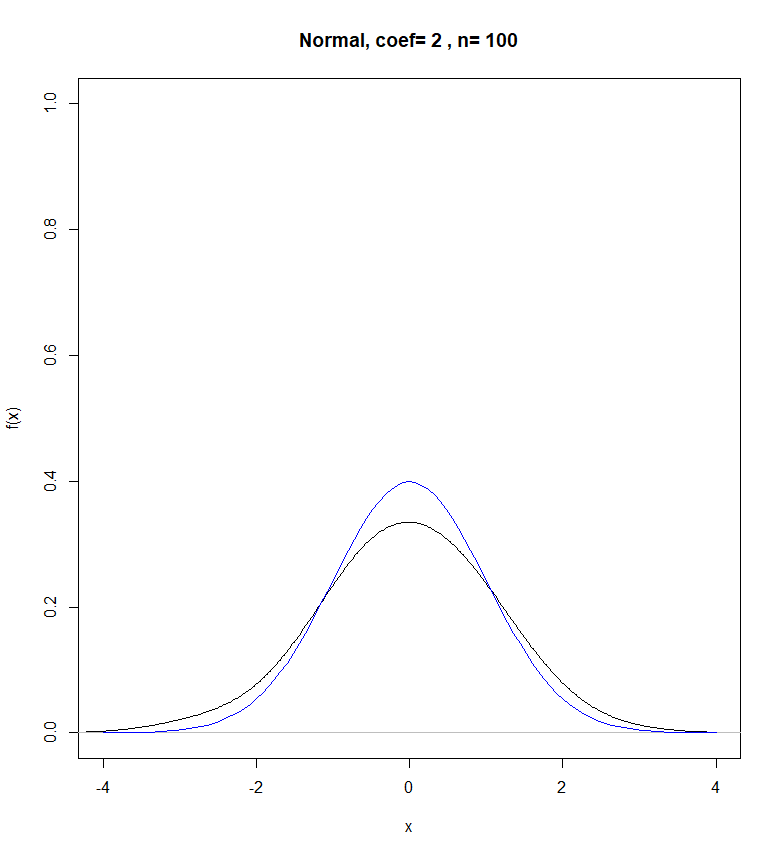
\includegraphics[width=\linewidth]{4f241c16-0b9d-43b3-b8ff-a9d53f649893.png}
  \caption{\(Norm, h=2h_n\)}
\endminipage
 \label{fig:norm100}
\end{figure}
\newpage
%%%%%%%%%%%%%%%%%%%%%%%%%%%%%%%%% pois
\subsubsection{Распределение Пуассона, n = 20}
\begin{figure}[!htb]
\minipage{0.32\textwidth}
  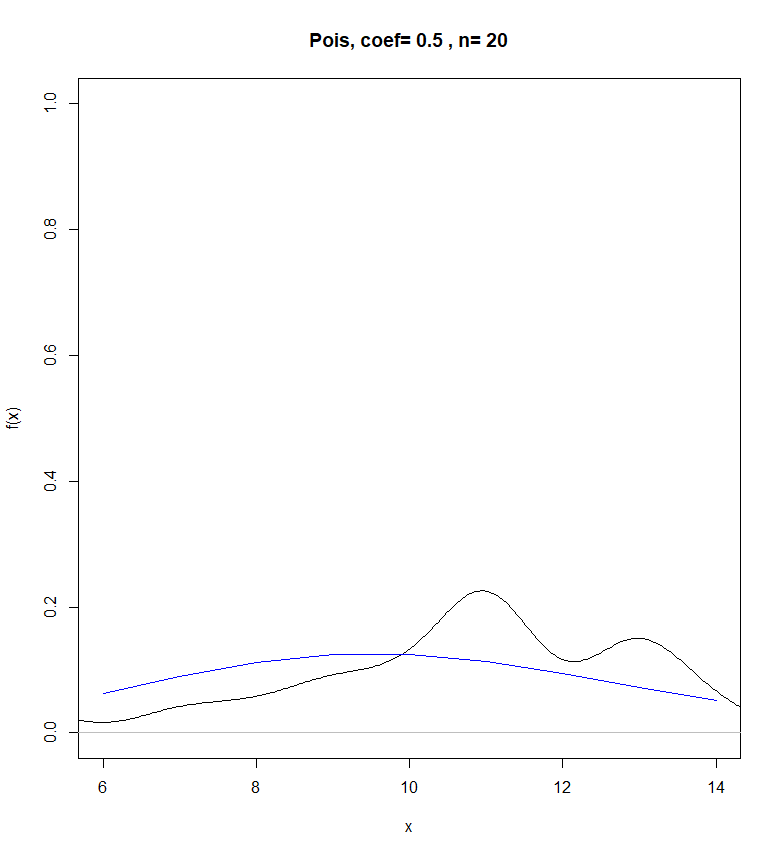
\includegraphics[width=\linewidth]{ad00dbd2-27dd-473c-b0e4-3c668bdfd333.png}
  \caption{\(Pois, h=h_n/2\)}
\endminipage\hfill
\minipage{0.32\textwidth}
  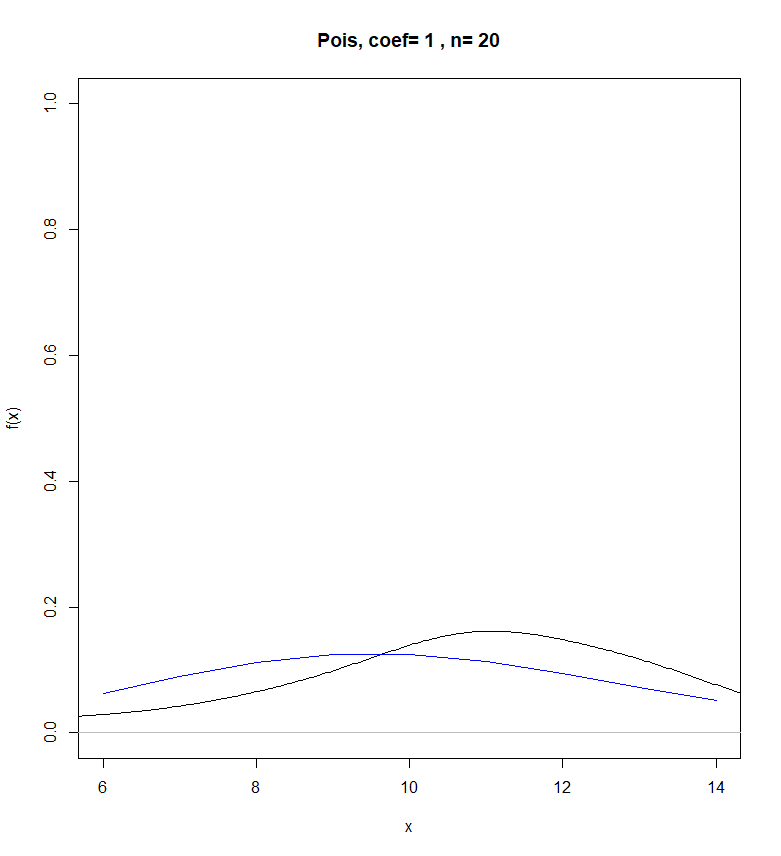
\includegraphics[width=\linewidth]{a1751869-88c8-4088-b8a1-705a964e0fc0.png}
  \caption{\(Pois, h=h_n\)}
\endminipage\hfill
\minipage{0.32\textwidth}
  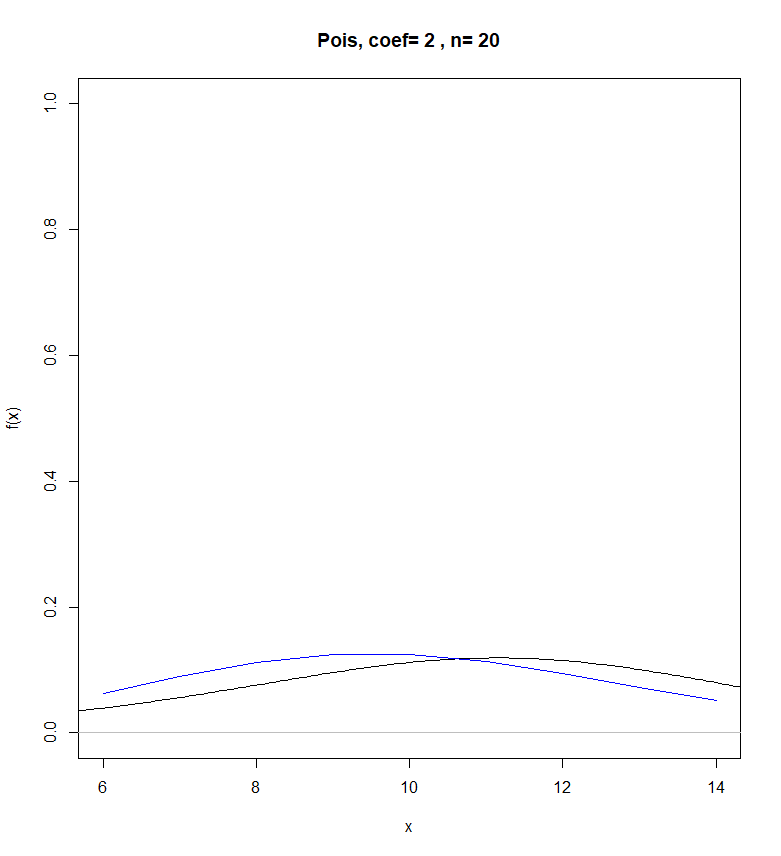
\includegraphics[width=\linewidth]{e8513016-7fad-4c79-a475-8ea79fc7fe1a.png}
  \caption{\(Pois, h=2h_n\)}
\endminipage
 \label{fig:pois20}
\end{figure}
\subsubsection{Распределение Пуассона, n = 60}
\begin{figure}[!htb]
\minipage{0.32\textwidth}
  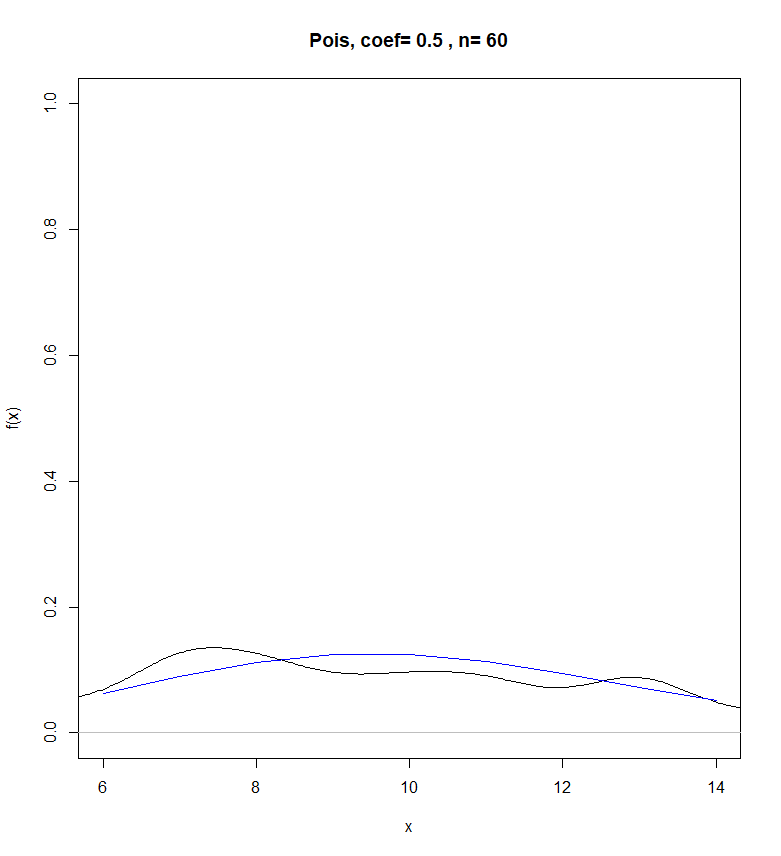
\includegraphics[width=\linewidth]{0854c84e-f0e7-4f27-addd-bd7ace1017fe.png}
  \caption{\(Pois, h=h_n/2\)}
\endminipage\hfill
\minipage{0.32\textwidth}
  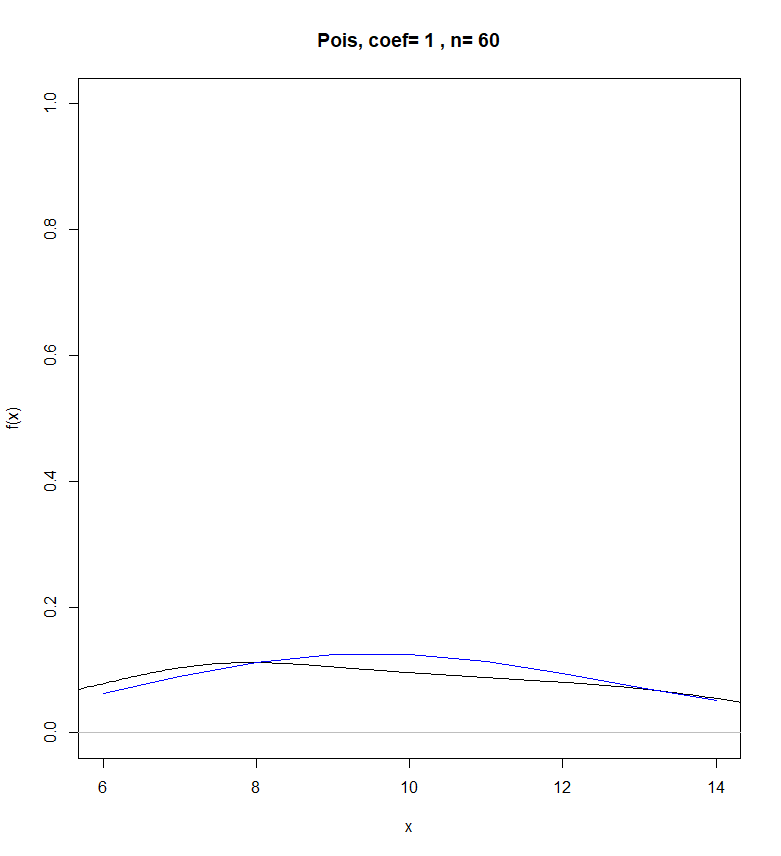
\includegraphics[width=\linewidth]{db1a4cd7-873c-4544-b80b-e1b11a5fe963.png}
  \caption{\(Pois, h=h_n\)}
\endminipage\hfill
\minipage{0.32\textwidth}
  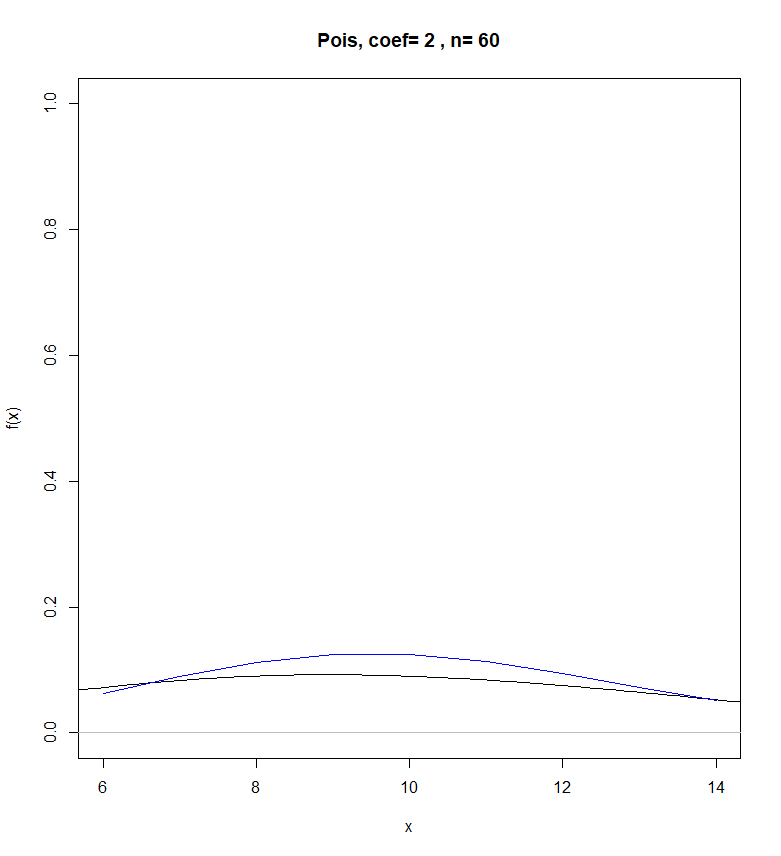
\includegraphics[width=\linewidth]{546fcecd-3367-4e34-843f-d515f8933130.png}
  \caption{\(Pois, h=2h_n\)}
\endminipage
 \label{fig:pois60}
\end{figure}
\subsubsection{Распределение Пуассона, n = 100}
\begin{figure}[!htb]
\minipage{0.32\textwidth}
  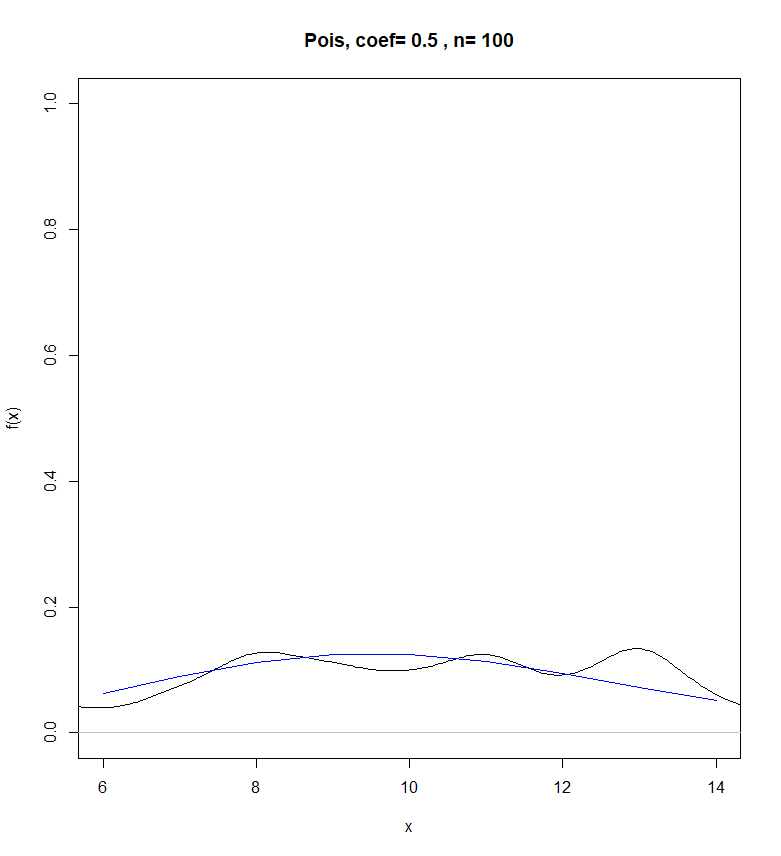
\includegraphics[width=\linewidth]{e1160f1a-bd95-488d-88c5-67489178feaf.png}
  \caption{\(Pois, h=h_n/2\)}
\endminipage\hfill
\minipage{0.32\textwidth}
  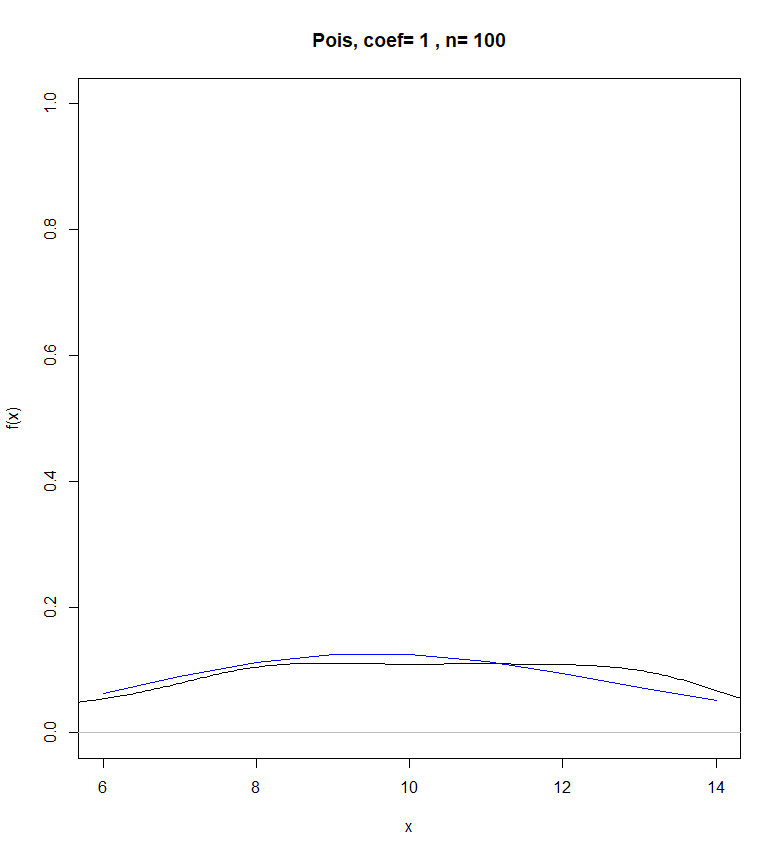
\includegraphics[width=\linewidth]{eddc73cd-a584-481c-8b9a-56ef8e2eb5ca.png}
  \caption{\(Pois, h=h_n\)}
\endminipage\hfill
\minipage{0.32\textwidth}
  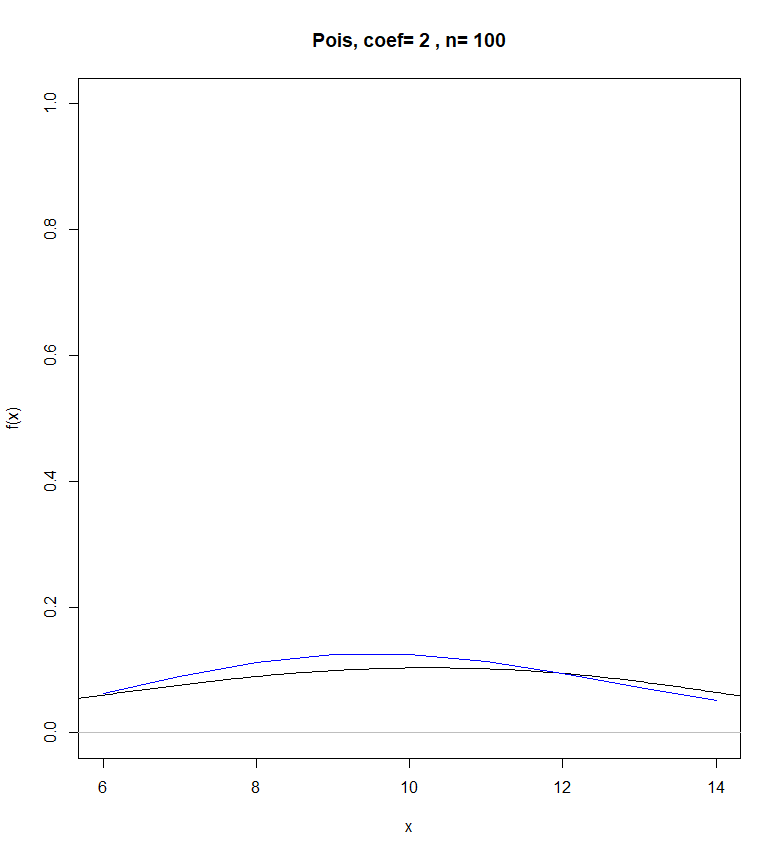
\includegraphics[width=\linewidth]{a706a25d-591b-4aa8-8d95-1e8f2b77228a.png}
  \caption{\(Pois, h=2h_n\)}
\endminipage
\label{fig:pois100}
\end{figure}
\newpage
%%%%%%%%%%%%%%%%%%%%%%%%%%%%%%%%% lapl
\subsubsection{Распределение Лапласа, n = 20}
\begin{figure}[!htb]
\minipage{0.32\textwidth}
  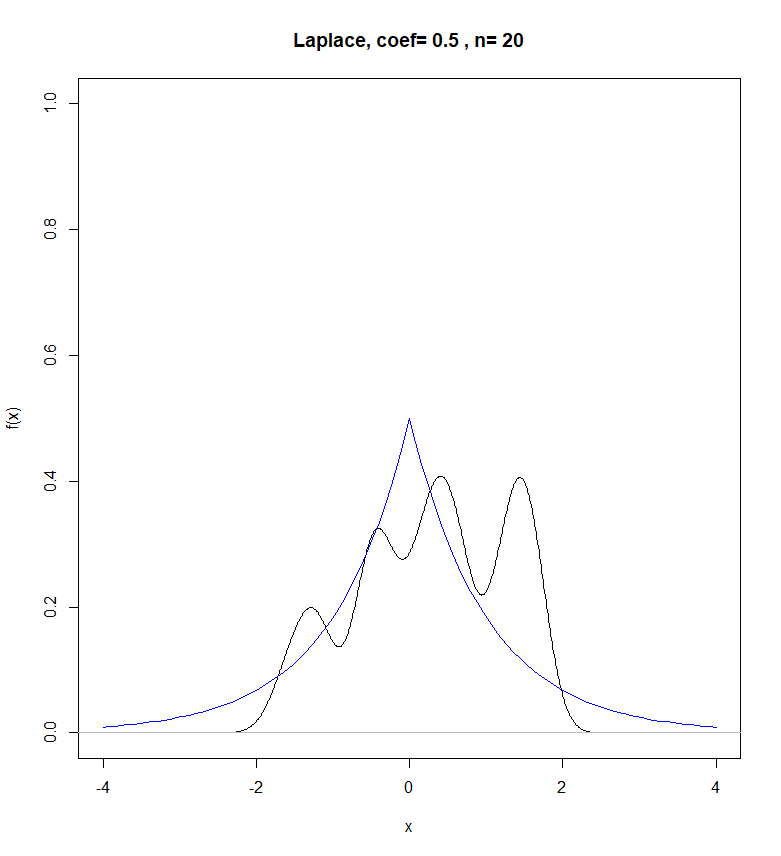
\includegraphics[width=\linewidth]{b9e0a0e8-3354-430d-b1aa-28428b8c32a3.png}
  \caption{\(Lapl, h=h_n/2\)}
\endminipage\hfill
\minipage{0.32\textwidth}
  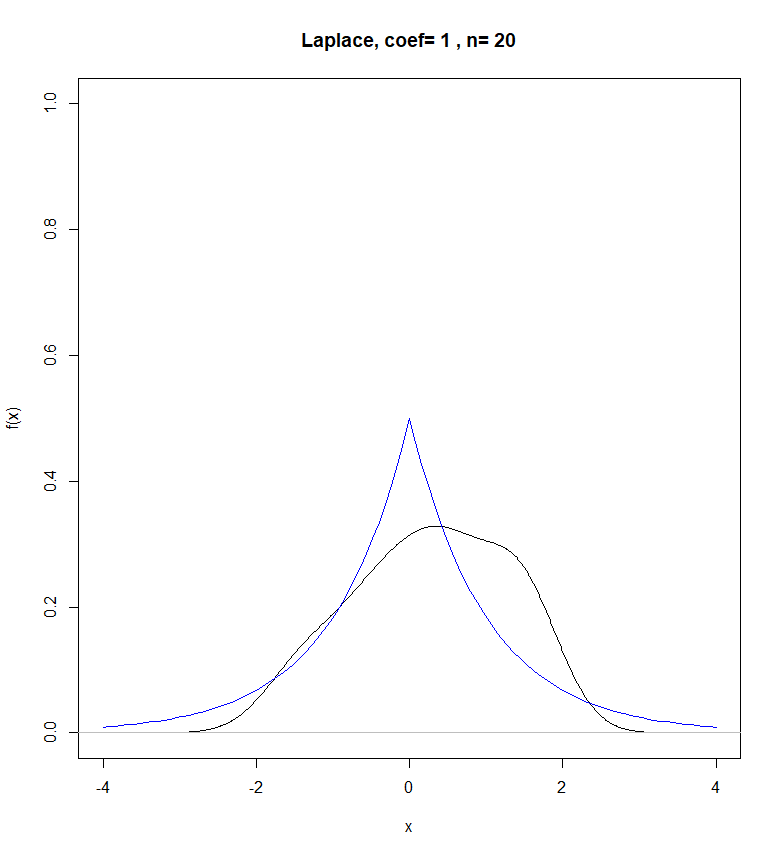
\includegraphics[width=\linewidth]{3516e1f7-4ddc-4cbc-92bc-cdc1f89e8bee.png}
  \caption{\(Lapl, h=h_n\)}
\endminipage\hfill
\minipage{0.32\textwidth}
  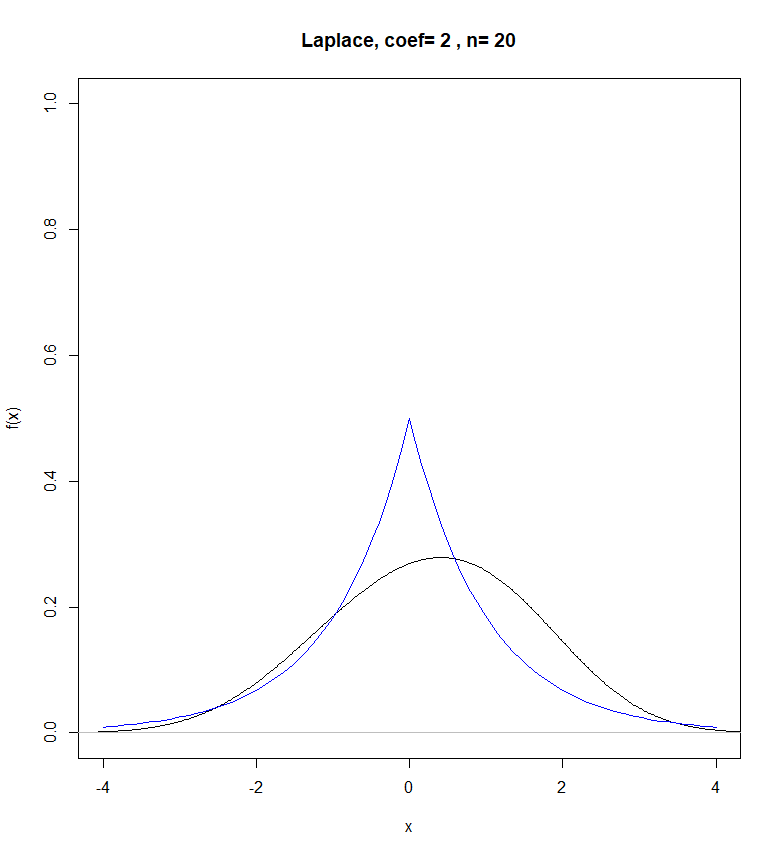
\includegraphics[width=\linewidth]{37f18a1a-18cb-47ed-98bb-bdf5b81253ca.png}
  \caption{\(Lapl, h=2h_n\)}
\endminipage
 \label{fig:lapl20}
\end{figure}
\subsubsection{Распределение Лапласа, n = 60}
\begin{figure}[!htb]
\minipage{0.32\textwidth}
  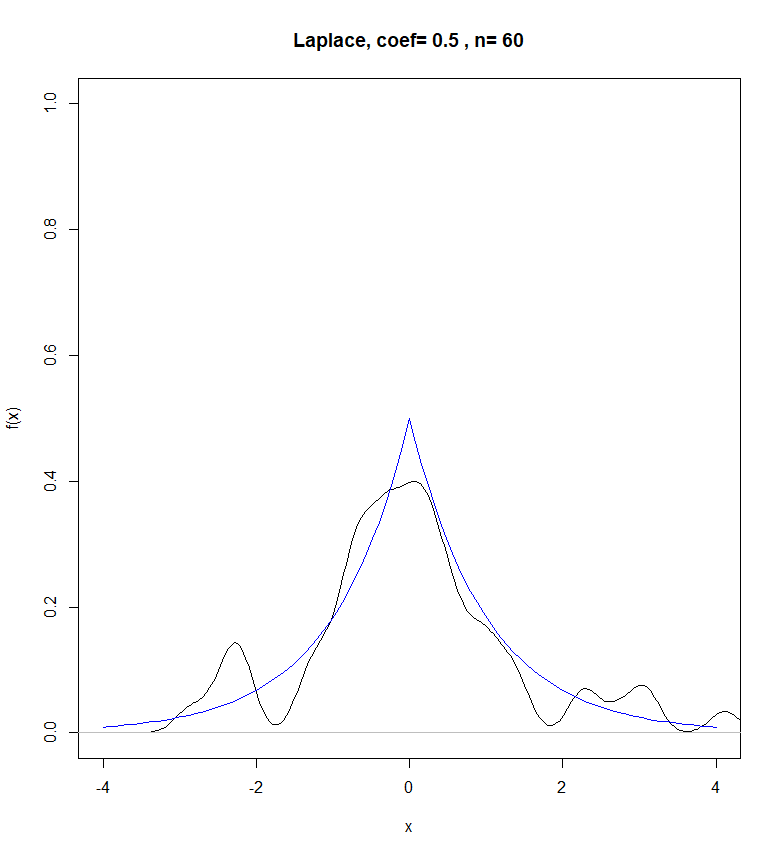
\includegraphics[width=\linewidth]{38c64432-e123-4fc2-b948-8c310ad2105b.png}
  \caption{\(Lapl, h=h_n/2\)}
\endminipage\hfill
\minipage{0.32\textwidth}
  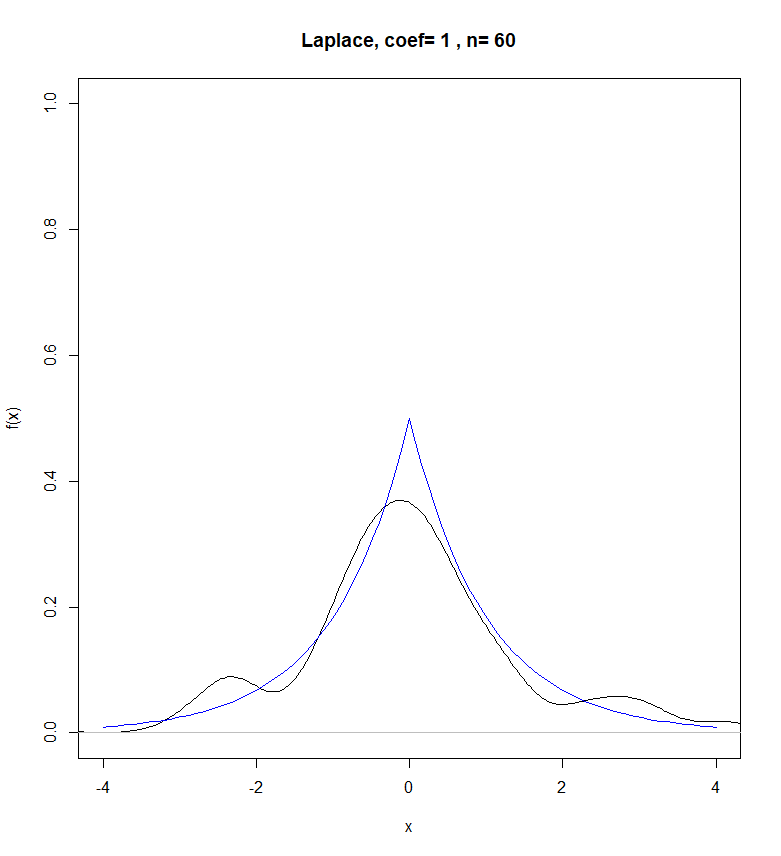
\includegraphics[width=\linewidth]{e5a2e003-2d91-4b0f-a9c4-0cfe8487088a.png}
  \caption{\(Lapl, h=h_n\)}
\endminipage\hfill
\minipage{0.32\textwidth}
  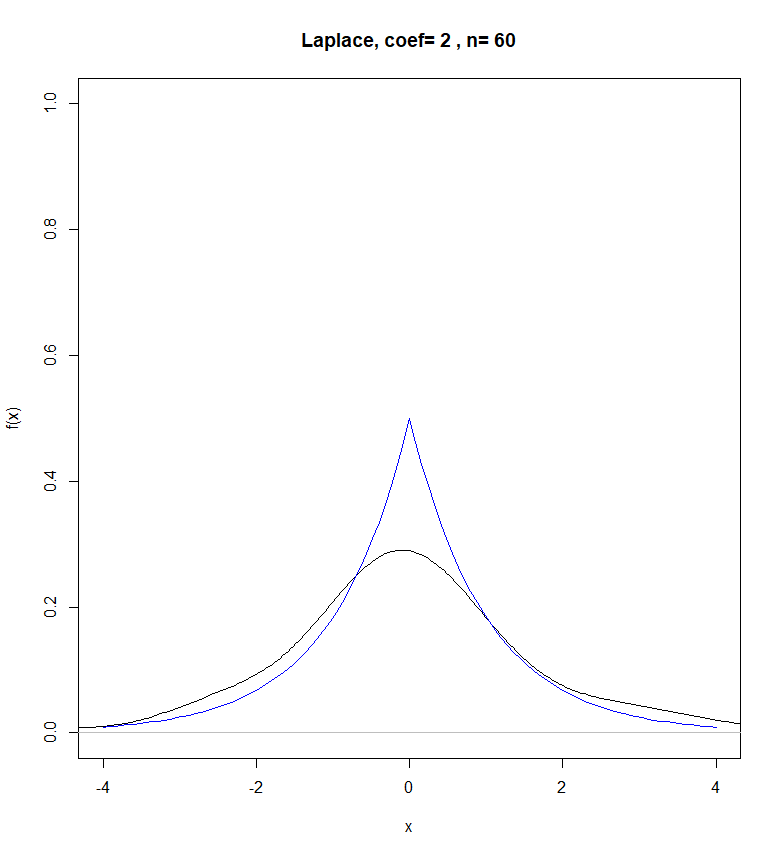
\includegraphics[width=\linewidth]{943756b7-6db2-4c4f-a8c9-c950b0b07192.png}
  \caption{\(Lapl, h=2h_n\)}
\endminipage
 \label{fig:lapl60}
\end{figure}
\subsubsection{Распределение Лапласа, n = 100}
\begin{figure}[!htb]
\minipage{0.32\textwidth}
  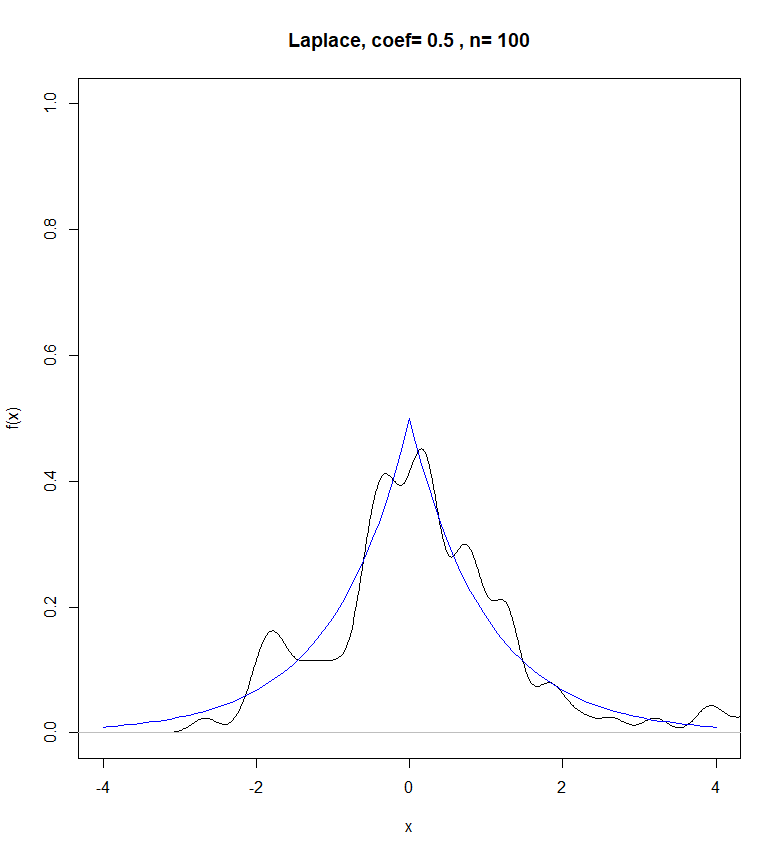
\includegraphics[width=\linewidth]{905608bc-2a14-4f89-b7ae-17b3d980630b.png}
  \caption{\(Lapl, h=h_n/2\)}
\endminipage\hfill
\minipage{0.32\textwidth}
  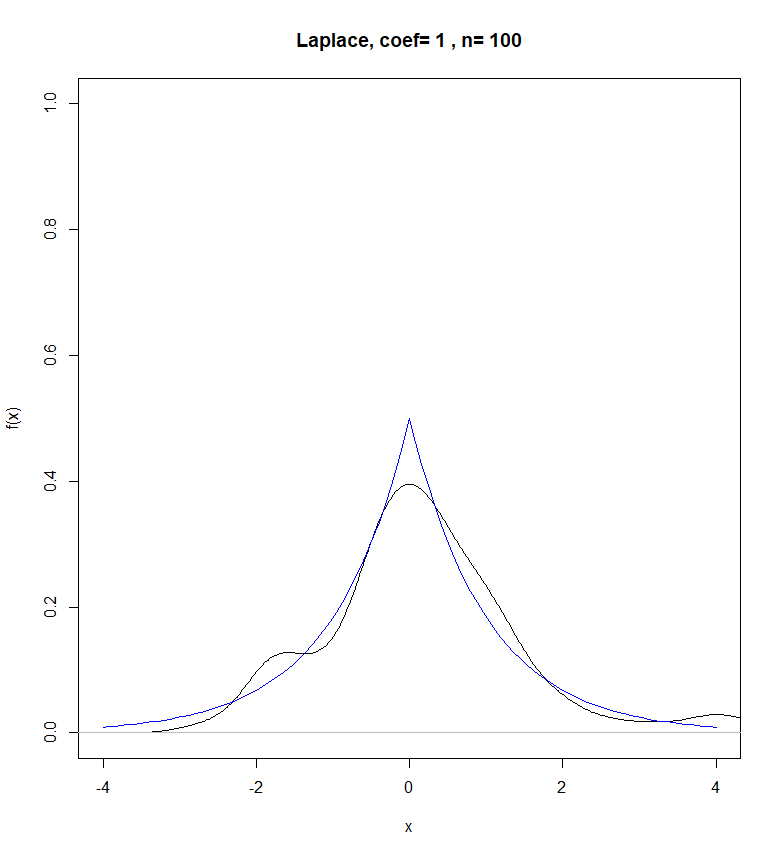
\includegraphics[width=\linewidth]{914d0421-5898-4543-b4aa-a6897763e13a.png}
  \caption{\(Lapl, h=h_n\)}
\endminipage\hfill
\minipage{0.32\textwidth}
  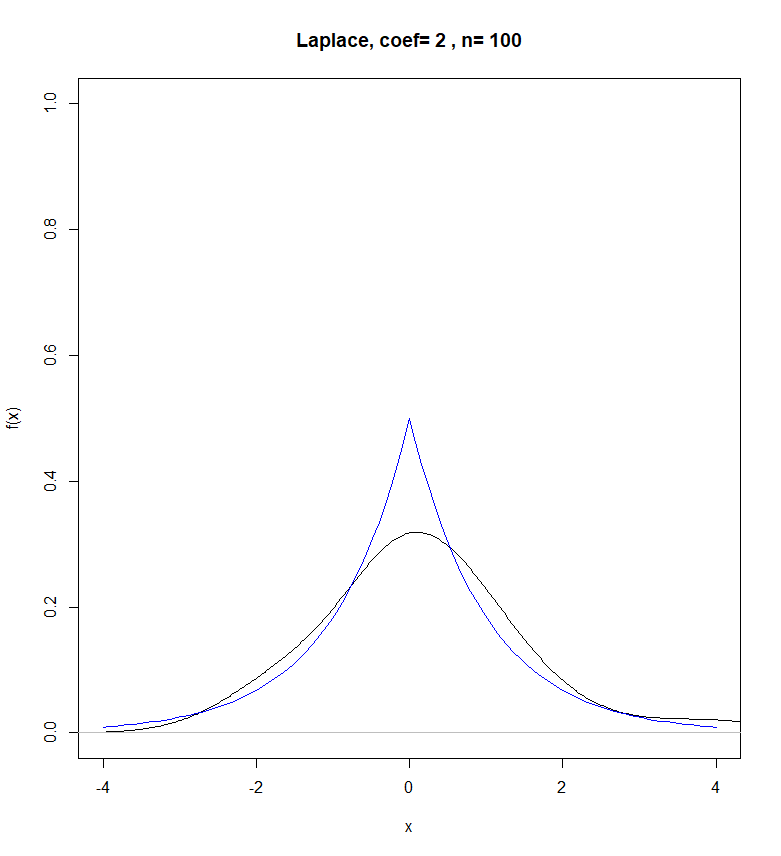
\includegraphics[width=\linewidth]{e1184b2a-9567-43ff-9fca-b25a87ffdb5c.png}
  \caption{\(Lapl, h=2h_n\)}
\endminipage
 \label{fig:lapl100}
\end{figure}
\newpage
%%%%%%%%%%%%%%%%%%%%%%%%%%%%%%%%% cauch
\subsubsection{Распределение Коши, n = 20}
\begin{figure}[!htb]
\minipage{0.32\textwidth}
  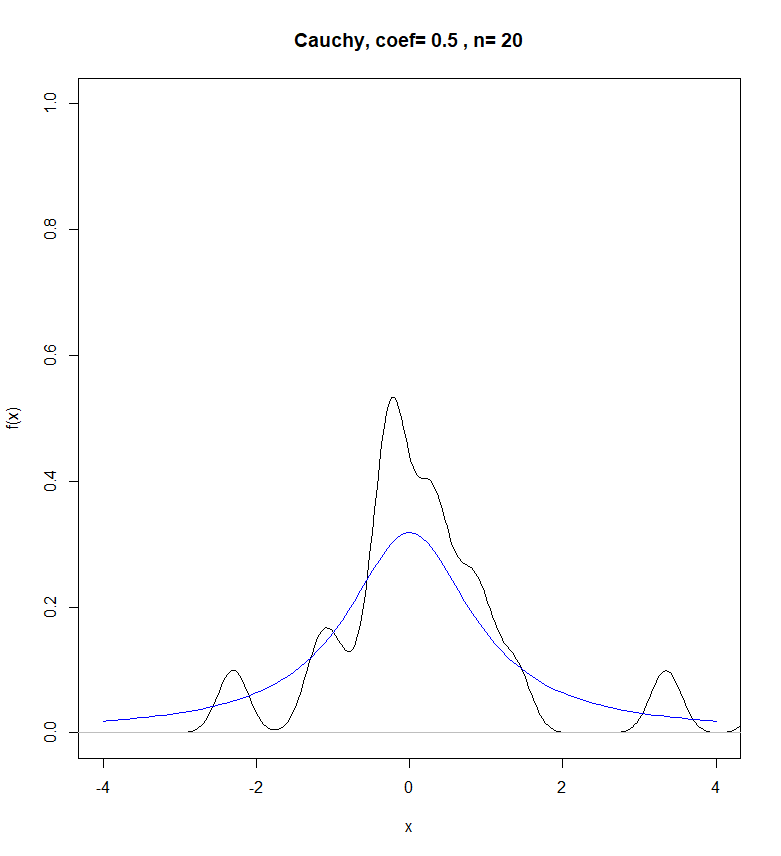
\includegraphics[width=\linewidth]{b1ef7dde-2104-401d-a808-e392496eaa92.png}
  \caption{\(Cauchy, h=h_n/2\)}
\endminipage\hfill
\minipage{0.32\textwidth}
  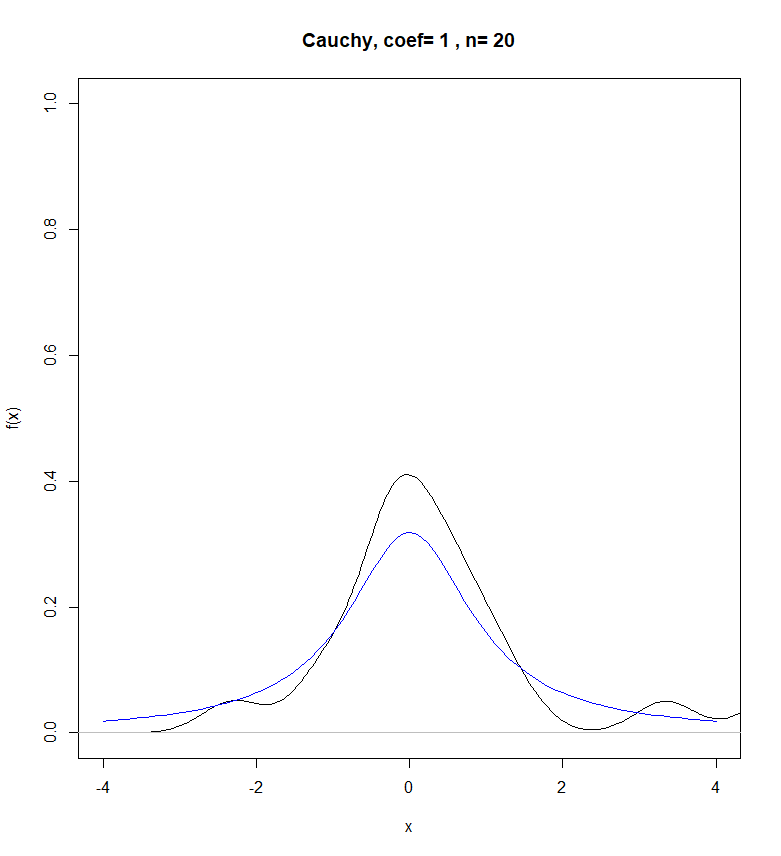
\includegraphics[width=\linewidth]{6011c99a-681a-46e9-a600-cbcf1a8d8599.png}
  \caption{\(Cauchy, h=h_n\)}
\endminipage\hfill
\minipage{0.32\textwidth}
  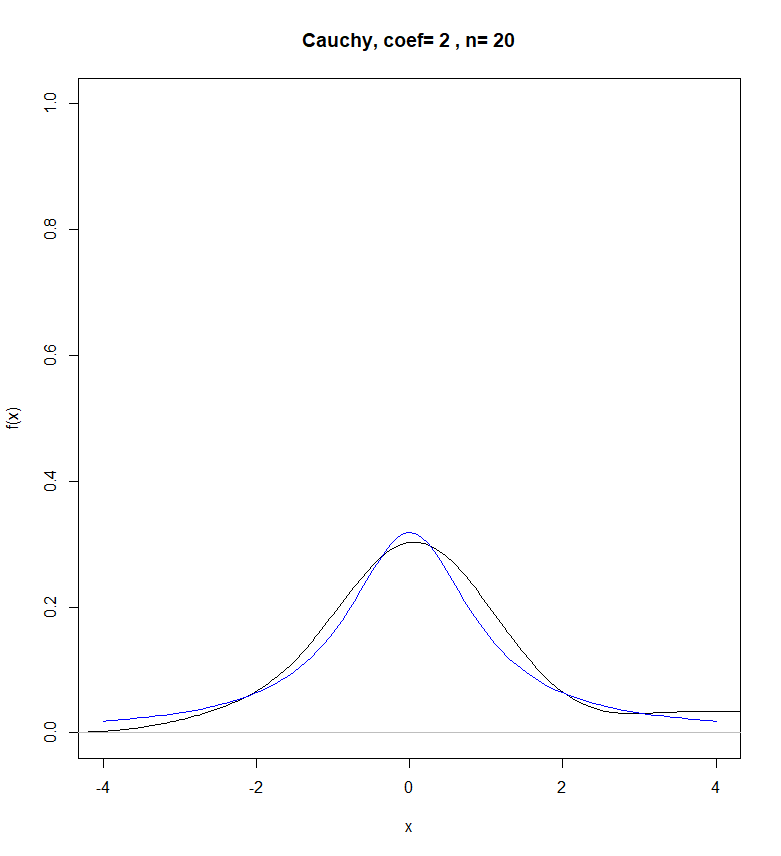
\includegraphics[width=\linewidth]{c3f3ef15-cc7a-4e59-9a93-c631e40745ee.png}
  \caption{\(Cauchy, h=2h_n\)}
\endminipage
\label{fig:cauch20}
\end{figure}
\subsubsection{Распределение Коши, n = 60}
\begin{figure}[!htb]
\minipage{0.32\textwidth}
  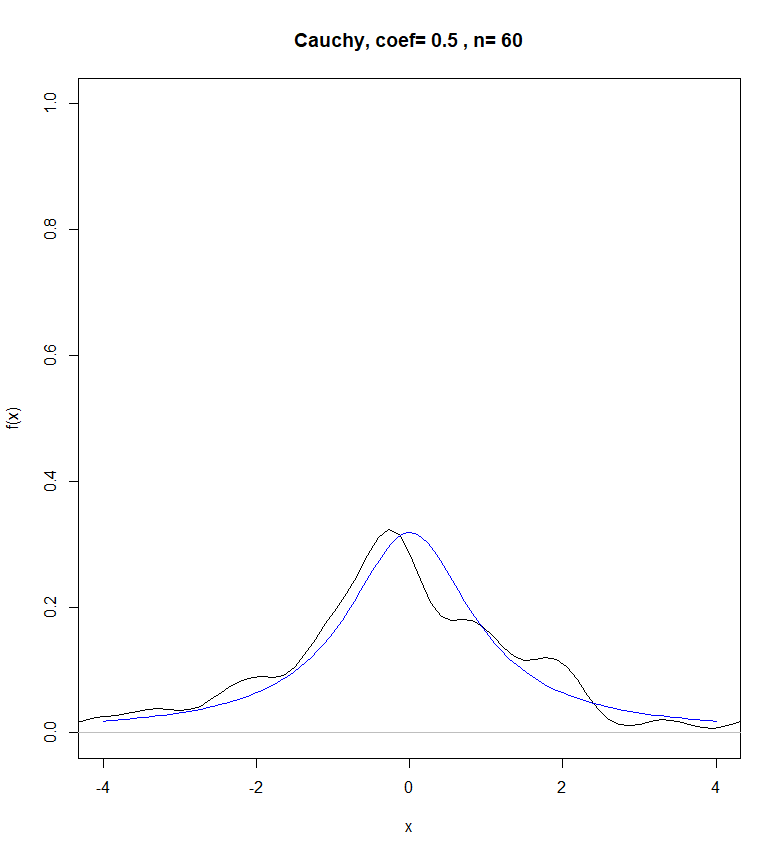
\includegraphics[width=\linewidth]{b47a0e01-fc98-4ffe-9a66-9e690477d373.png}
  \caption{\(Cauchy, h=h_n/2\)}
\endminipage\hfill
\minipage{0.32\textwidth}
  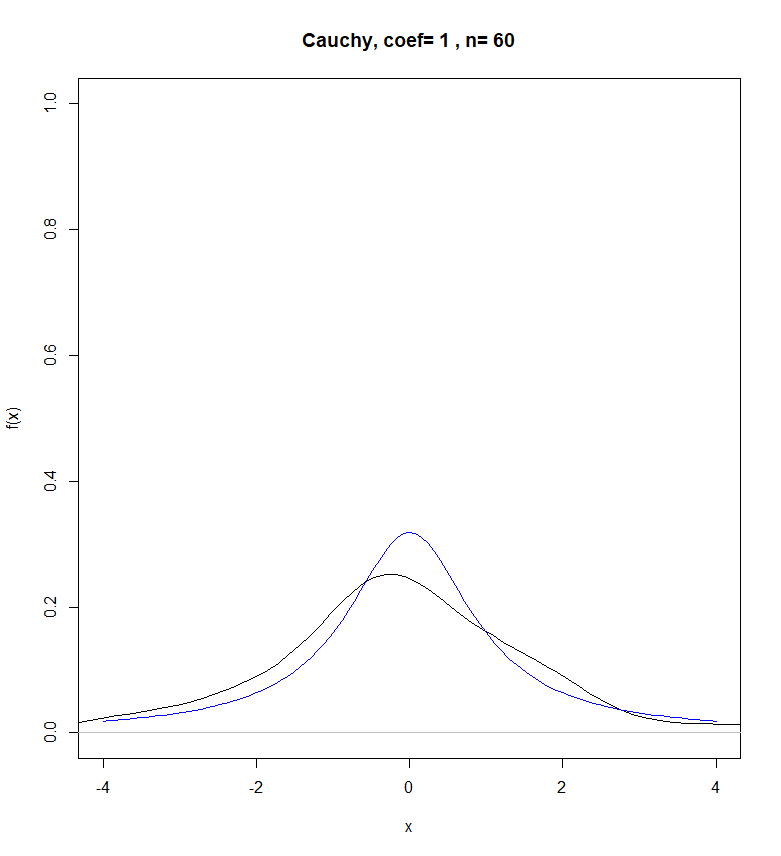
\includegraphics[width=\linewidth]{b92ad9eb-6ebb-48a9-958e-3daae8928b28.png}
  \caption{\(Cauchy, h=h_n\)}
\endminipage\hfill
\minipage{0.32\textwidth}
  \includegraphics[width=\linewidth]{fc60b29b-e9fc-45ed-94dd-578ce6840ae3.png}
  \caption{\(Cauchy, h=2h_n\)}
\endminipage
\label{fig:cauch60}
\end{figure}
\newpage
\subsubsection{Распределение Коши, n = 100}
\begin{figure}[!htb]
\minipage{0.32\textwidth}
  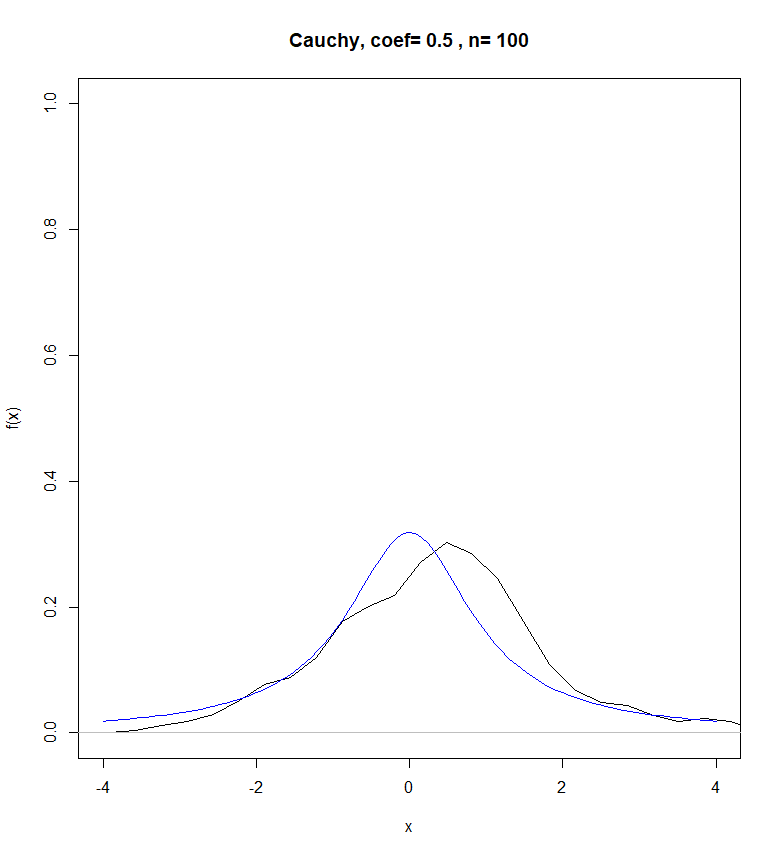
\includegraphics[width=\linewidth]{57dd9abd-0445-4de9-9a55-f2292c08e248.png}
  \caption{\(Cauchy, h=h_n/2\)}
\endminipage\hfill
\minipage{0.32\textwidth}
  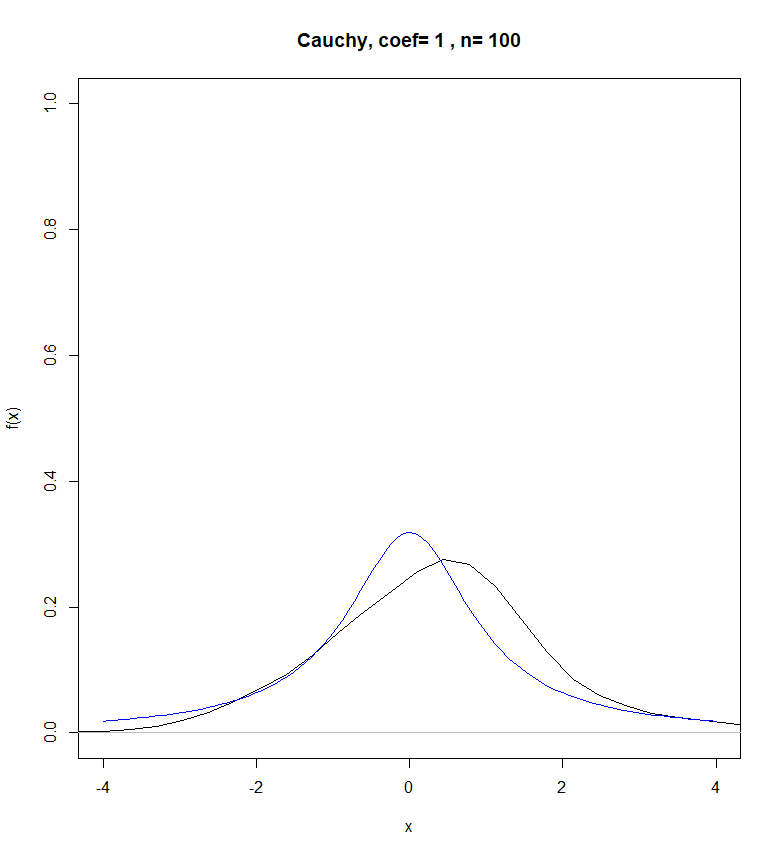
\includegraphics[width=\linewidth]{24d7cc67-1b8b-465e-b840-d21e3b57ec84.png}
  \caption{\(Cauchy, h=h_n\)}
\endminipage\hfill
\minipage{0.32\textwidth}
  \includegraphics[width=\linewidth]{ca85b8ed-906d-4ed7-a79f-1b4d9c6365b1.png}
  \caption{\(Cauchy, h=2h_n\)}
\endminipage
\label{fig:cauch100}
\end{figure}
\newpage
%%%%%%%%%%%%%%%%%%%%%%%%%%%%%%%%%%%% unif
\subsubsection{Равномерное распределение, n = 20}
\begin{figure}[!htb]
\minipage{0.32\textwidth}
  \includegraphics[width=\linewidth]{bc996065-4196-4de4-83d8-add7bb3c388e.png}
  \caption{\(Unif, h=h_n/2\)}
\endminipage\hfill
\minipage{0.32\textwidth}
  \includegraphics[width=\linewidth]{c23086d6-297c-4dce-96ad-2cf57792292d.png}
  \caption{\(Unif, h=h_n\)}
\endminipage\hfill
\minipage{0.32\textwidth}
  \includegraphics[width=\linewidth]{eba91e91-6201-4047-9af3-6bde67e565ef.png}
  \caption{\(Unif, h=2h_n\)}
\endminipage
\label{fig:unif20}
\end{figure}
\subsubsection{Равномерное распределение, n = 60}
\begin{figure}[!htb]
\minipage{0.32\textwidth}
  \includegraphics[width=\linewidth]{ea519b16-ed3d-4ff0-8325-309f017ba219.png}
  \caption{\(Unif, h=h_n/2\)}
\endminipage\hfill
\minipage{0.32\textwidth}
  \includegraphics[width=\linewidth]{2a39f09e-cdb7-4f60-b339-2257802d8f66.png}
  \caption{\(Unif, h=h_n\)}
\endminipage\hfill
\minipage{0.32\textwidth}
  \includegraphics[width=\linewidth]{23525562-6126-4612-bccf-28715d653f86.png}
  \caption{\(Unif, h=2h_n\)}
\endminipage
 \label{fig:unif60}
\end{figure}
\subsubsection{Равномерное распределение, n = 100}
\begin{figure}[!htb]
\minipage{0.32\textwidth}
  \includegraphics[width=\linewidth]{43773d42-e954-4442-b4f8-3721c59853fa.png}
  \caption{\(Unif, h=h_n/2\)}
\endminipage\hfill
\minipage{0.32\textwidth}
  \includegraphics[width=\linewidth]{ba399cb1-c98d-4753-b5da-9e141d399159.png}
  \caption{\(Unif, h=h_n\)}
\endminipage\hfill
\minipage{0.32\textwidth}
  \includegraphics[width=\linewidth]{a0461f26-0998-48eb-8d7e-ae35396190d6.png}
  \caption{\(Unif, h=2h_n\)}
\endminipage
\label{fig:unif100}
\end{figure}
\newpage

\section{Обсуждение}
Из представленных графиков видно, что при увеличении размеров выборки эмпирические функции распределения приближаются к реальным функциям распределения соответствующих распределений.\\
Ядерная оценка плотности распределения также приближается к теоретической плотности распределения при увеличении выборки.\\
При выборе сглаживающего параметра по правилу Сильвермана характер поведения ядерной оценки плотности будет сбалансирован: не сильно «волнистая», но и не сильно «гладкая».  Данное значение параметра можно использовать как стартовое для корректировки характера поведения ядерной оценки. Для получения более гладкой кривой можно увеличить параметр, а для получения более резких скачков и переходов – соответственно уменьшить.

\section{Приложения}
Репозиторий на Github с кодом лабораторной работы:\\
\url{https://github.com/VsevolodMelnikov/Math_Stat/tree/master/lab4}

\end{document}
